\documentclass[10pt]{article}
%\usepackage[utf8x]{inputenc}

%\usepackage{html}   %  *always* load this for LaTeX2HTML
\usepackage{makeidx}
\usepackage[usenames,dvipsnames]{xcolor}
\usepackage[colorlinks=true, citecolor=green!60!black, linkcolor=red!60!black, urlcolor=purple!60!black, filecolor=magenta!30!black]{hyperref}
\usepackage[pdftex]{graphicx}
\usepackage{setspace}
\usepackage{calc}
\usepackage{colortbl}
\usepackage{verbatim}
\usepackage{ifthen}
\usepackage[labelfont=bf]{caption} 
\usepackage{fancyhdr}
\usepackage{extramarks}

\usepackage[sort,compress,numbers]{natbib}
%\setlength{\natbibspacing}{0.2em}

%\usepackage{customsections}     %reformats chapter/section titles 
%\usepackage{fullpage}

\setlength{\captionmargin}{4ex}
\setlength{\headheight}{12pt}       % I need a larger header for the accent in my name
\setlength{\headsep}{15pt}
\setlength{\topmargin}{25pt}
\setlength{\footskip}{40pt}         % adds a bit more space between bottom of text/page number
\setlength{\hoffset}{0.125in}
%creates a length that shifts page away from the inside edge in double-sided printing
\newlength{\insideshift}
\setlength{\insideshift}{0.8in}
% adjusts textwidth/height based on above sizes
\setlength{\textwidth}{\paperwidth-2in-2\hoffset-\insideshift}
\setlength{\textheight}{\paperheight-2in-2\voffset-\topmargin-\headheight-\headsep-\footskip}   % makes bottom of footer at 1in+\voffset
\setlength{\headwidth}{\textwidth}      % adjusts header to match textwidth
\setlength{\evensidemargin}{0.5\insideshift}
\setlength{\oddsidemargin}{0.5\insideshift}


\usepackage{listings}
\lstset{  language=C++,  basicstyle=\ttfamily\small,  keywordstyle=\color{blue!70!black},  identifierstyle=,  commentstyle=\color{green!50!black}\itshape\ttfamily,
          stringstyle=\color{red!60!black}\ttfamily,  showstringspaces=false,  backgroundcolor=\color{gray!5},  fillcolor=\color{gray!5}, rulesepcolor=\color{gray!5},
          rulecolor=\color{black}, framexleftmargin=4ex, framexrightmargin=4ex, framexbottommargin=0.5em, framextopmargin=0.25em, xleftmargin=4ex, xrightmargin=4ex,
          columns=fixed, basewidth={1.2ex,1.5ex}, fontadjust=true, numbers=left, numberstyle=\tiny\color{gray!80}, stepnumber=1, numbersep=4ex, 
          escapeinside={/*@}{@*/}, frameshape={n}{}{}{nyn}
}

\newcommand{\lstquick}[1]{\lstinline[language=C++,basicstyle=\ttfamily\color{black!90},keywordstyle=\color{blue!60!black!90},columns=fixed,fontadjust=true,identifierstyle=, commentstyle=\color{green!50!black}\itshape\ttfamily,stringstyle=\color{red!60!black}\ttfamily,basewidth={1.2ex,1.5ex}]{#1}}

\usepackage{lstskipnumbers}
\lstnewenvironment{lstshortblock}
    {\lstset{ language=C++, numbers=none,backgroundcolor=\color{gray!5}, xleftmargin=8ex, xrightmargin=6ex, framexleftmargin=4ex, framexrightmargin=2ex,
              frameshape={nyn}{}{}{nnn},
              basicstyle=\ttfamily\small, keywordstyle=\color{blue!70!black}, identifierstyle=, commentstyle=\color{green!50!black}\itshape\ttfamily,
              stringstyle=\color{red!60!black}\ttfamily, columns=fixed, basewidth={1.2ex,1.5ex}, fontadjust=true  } }
    {}

\lstnewenvironment{lstplainblock}
    {\lstset{ language=C++, numbers=none, backgroundcolor=\color{white}, xleftmargin=4ex, xrightmargin=0ex, framexleftmargin=0ex, framexrightmargin=0ex,
              frame=none,
              basicstyle=\ttfamily\small, keywordstyle=\color{blue!70!black}, identifierstyle=, commentstyle=\color{green!50!black}\itshape\ttfamily,
              stringstyle=\color{red!60!black}\ttfamily, columns=fixed, basewidth={1.2ex,1.5ex}, fontadjust=true  } }
    {}

%\captionsetup[lstlisting]{singlelinecheck=false, labelfont={blue}, textfont={blue}}
\DeclareCaptionFont{white}{\color{white}}
\DeclareCaptionFormat{listing}{\colorbox{gray!80}{\parbox{\textwidth-6pt}{\hspace{\parindent}#1#2#3}}}
\captionsetup[lstlisting]{format=listing,labelfont=white,textfont=white, singlelinecheck=false, margin=0pt, font={bf,small}}

\newlength{\tmplength}
\newlength{\codemargin}         \newlength{\codeindent}
\setlength{\codemargin}{0pt}    \setlength{\codeindent}{0in}
\newcommand{\codelabel}[1]{\settowidth{\tmplength}{\texttt{#1}x}\parbox[t]{\tmplength}{\texttt{#1}:}\hfill}
\newcommand{\longitem}[1]{\item[#1] \parbox{\textwidth-\tmplength-\labelsep}{\hfill}\\}
\newenvironment{codelist}
   {\begin{list}{} %
      {\renewcommand{\makelabel}{\codelabel}
       \setlength{\labelwidth}{11ex}
       \setlength{\labelsep}{1ex}
       \setlength{\itemsep}{0.2em}
       \setlength{\leftmargin}{16ex}
       \setlength{\rightmargin}{4ex}
      }
   }
   {\end{list}}

\newenvironment{fdescription}{
        \small
        \settowidth{\tmplength}{Workspace:}
        \begin{tabular}{@{\hspace*{8ex}}p{\tmplength}@{\hspace*{2ex}}p{\textwidth-\tmplength-18ex}@{\hspace*{8ex}}}
    }
    {   \end{tabular}   }
\newcommand{\fdbottom}{\vspace*{-0.5em}

                       \noindent\hspace*{4ex}\rule{\textwidth-8ex}{0.5pt}\hfill
                       \vspace*{1em}}

\settowidth{\tmplength}{\texttt{template <class A, class B>}}
\newlength{\dodgethis} 
\newcommand{\templatecode}[4]{ {\small
    \settowidth{\tmplength}{\texttt{#2}}
    \settowidth{\dodgethis}{\texttt{doublexxx}}
    \setlength{\tmplength}{\dodgethis-\tmplength}
    \noindent \hspace*{2ex}\parbox[t]{\textwidth-2ex}{\code{#1}}\\
    \noindent \hspace*{2ex}\parbox[t]{\dodgethis}{\hspace*{\tmplength}\code{#2}}\hspace*{1.5ex}\parbox[t]{\textwidth-\dodgethis-7ex}{\code{#3}\\[0.2em] #4}
    \bigskip

 }}
\newcommand{\templatecodecont}[4]{ {\small
    \settowidth{\tmplength}{\texttt{#2}}
    \settowidth{\dodgethis}{\texttt{doublexxx}}
    \setlength{\tmplength}{\dodgethis-\tmplength}
    \noindent \hspace*{2ex}\parbox[t]{\dodgethis}{\hspace*{\tmplength}\code{#2}}\hspace*{1.5ex}\parbox[t]{\textwidth-\dodgethis-7ex}{\code{#3}\\[0.2em] #4}
    \bigskip

 }}

%\newcommand{\codelabel}[1]{\parbox[t]{\textwidth-2\codemargin}{\setlength{\parindent}{-5ex}\setlength{\leftskip}{5ex}\texttt{#1}}}
\newlength{\leftshift}
\newlength{\bodyindent}
\newlength{\ccwordlength}
\setlength{\bodyindent}{0.5in}
\newcommand{\codeitem}[2]{\item[#1] \lstquick{#2}\hfill\\}
\newcommand{\compactcodelabel}[1]{  \settowidth{\ccwordlength}{\texttt{#1}x}
                                    \setlength{\leftshift}{\ccwordlength}
                                    \addtolength{\leftshift}{\leftmargin}
                                    \addtolength{\leftshift}{-\bodyindent}
                                    \addtolength{\leftshift}{1.5ex}
                                    \hspace*{-\leftshift}\parbox[t]{\ccwordlength}{\lstquick{#1}}        }
\newenvironment{compactcodelist}
   {\begin{list}{} %
      {\setlength{\labelwidth}{0.2in}
       \setlength{\labelsep}{0in}
       \setlength{\itemsep}{0in}
       \setlength{\leftmargin}{\bodyindent}
       \setlength{\rightmargin}{0pt}
       \renewcommand{\makelabel}{\compactcodelabel}
      }
   }
   {\end{list}}


\newcommand{\var}[1]{{\slshape #1}}
\newlength{\loadfunclen}
\newcommand{\deftypefn}[3]{ \settowidth{\loadfunclen}{[#1]}
                            \noindent\parbox{\textwidth-\loadfunclen}{\texttt{#2 #3}}\parbox{\loadfunclen}{[#1]}}
\newcommand{\deftypefnx}[3]{\deftypefn{#1}{#2}{#3}}

\newlength{\texitablemargin}
\newlength{\texiitemindent}
\setlength{\texitablemargin}{0.8in}
\setlength{\texiitemindent}{2ex}
\newcommand{\texilabel}[1]{\parbox{\texitablemargin}{\hspace*{\texiitemindent}\texttt{#1}}}
\newenvironment{texitable}
   {\begin{list}{} %
      {\renewcommand{\makelabel}{\texilabel}
       \setlength{\labelwidth}{\texitablemargin}
       \setlength{\labelsep}{0pt}
       \setlength{\itemsep}{0.2em}
       \setlength{\leftmargin}{\texitablemargin}
       \setlength{\rightmargin}{4ex}
      }
   }
   {\end{list}}

\newenvironment{texiexample}{\vspace*{-0.5em}\verbatim 
                                        }
                            {\endverbatim \vspace*{-0.5em}}


\usepackage{amsmath}
\usepackage{amsthm}

\newtheoremstyle{cool}% name of the style to be used
  {3pt}% measure of space to leave above the theorem. E.g.: 3pt
  {3pt}% measure of space to leave below the theorem. E.g.: 3pt
  {\itshape}% name of font to use in the body of the theorem
  {0pt}% measure of space to indent
  {\bfseries}% name of head font
  {:}% punctuation between head and body
  {0.5em}% space after theorem head; " " = normal interword space
  {}% Manually specify head

\theoremstyle{cool}
\newtheorem*{problem}{Problem}

%opening
\title{\texttt{mtpsd} Documentation}
\author{C.~Antonio S\'anchez}

\newcommand{\code}[1]{\lstquick{#1}}

\renewcommand\listtablename{Tables}
\renewcommand\listfigurename{Figures}

\makeindex

\newcommand{\sectiontitle}{}
\newcommand{\newsection}[1]{\renewcommand{\sectiontitle}{#1}\markboth{\scshape \sectiontitle}{}\section{\sectiontitle}\markboth{\scshape \sectiontitle}{} }

\fancypagestyle{plain}{
    \fancyhf{}
    \lhead{}
    \lfoot{}
    \cfoot{\thepage}
    \renewcommand{\headrulewidth}{0pt}
    \renewcommand{\footrulewidth}{0pt}    
}
\fancypagestyle{contents}{
    \renewcommand{\headrulewidth}{0.5pt}
    \lhead{\firstleftmark}
    \rhead{}
    \lfoot{}
    \cfoot{\thepage}
}
\fancypagestyle{body}{
    \renewcommand{\headrulewidth}{0.5pt}
    \lhead{\firstleftmark}
    \rhead{\rightmark}
    %\rhead{\ifthenelse{\equal{\rightmark}{}}{}{\thesection\hspace{1ex}\rightmark}}
    \lfoot{}
    \cfoot{\thepage}
}

\begin{document}

\maketitle
\thispagestyle{empty}

\begin{abstract}
\noindent The \code{mtpsd} library contains a collection of functions for estimating the power spectral density (PSD) of a one-dimensional time-series, along with its statistical properties, using Thomson's multitaper (MT) method.  This includes adaptive weighting, confidence intervals, an F-test for significant frequencies, and methods for computing the special tapers: discrete prolate spheroidal sequences.  This library is written in C++, and depends on LAPACK and FFTW3.  Also included in the package are Octave dynamical extensions (oct-files) to interface with the library, and a command-line executable to compute tapers.
\end{abstract}
\bigskip

\begin{center}
    \copyright~C.~Antonio S\'anchez 2012
\end{center}

\newpage

\pagenumbering{roman}

\pagestyle{contents}

\tableofcontents
\listoftables
\lstlistoflistings
\listoffigures

\newpage

\section*{Preface}
\renewcommand{\sectiontitle}{Preface}
\markboth{\scshape \sectiontitle}{}
\addcontentsline{toc}{section}{Preface}
The intent of this documentation is two-fold:
\begin{itemize}
    \item to describe the use of the classes and methods contained in the 
        \texttt{mtpsd} library, and
    \item to explain the underlying mechanisms and the reasoning behind them.
\end{itemize}
In my (short and limited) experience, I've learned to be wary of academic tools
that don't explain precisely the way they work behind-the-scenes.  When 
something isn't behaving as expected, one is often stuck examining the source 
code, trying to decipher the algorithms the author used (or \emph{tried to} 
use).  It is my hope that this document is clear about how each method does 
what it does.  Unfortunately, this meant I had to include a Theory section, 
where I could put the equations involved.  For this section, it is assumed 
that the reader is somewhat familiar with frequency analysis, and has at least 
heard of David Thomson's multitaper technique.  If not, excellent sources of 
information are Thomson's seminal paper on the multitaper method 
\cite{thomson:multitaper}, and Percival and Walden's fundamental text on 
spectral analysis \cite{percival:multitaper}.

The original motivation for this project was, unfortunately, the result of an 
academic tool not behaving as expected.  While taking a course on statistical 
signal processing (taught by Thomson), I found that the confidence intervals 
produced by \textsc{Matlab} for an adaptively weighted spectrum estimate seemed
to match too closely to those for uniform weighting.  At the time, I just found
it curious, but decided not to investigate.  It wasn't until recently, when I 
needed the functionality in the open-source GNU Octave, that I had cause to 
look into it.

The Octave signal processing toolbox does not include the multitaper technique,
and I was not able to find a suitable (open-source) replacement.  So, I began 
coding my own, comparing results with \textsc{Matlab} to make sure the two were
consistent.  For eigenvalue weighting, the two results were close, but would 
not match exactly.  For adaptive weighting, my confidence intervals were quite 
a bit larger, which reminded me of Thomson's course.  This led me to examine 
the source code for \textsc{Matlab}'s \texttt{pmtm} function, to see exactly 
what was being returned.  I found the following `bugs':
\begin{itemize}
    \item For eigenvalue weighting with $K$ tapers, the weights are 
        approximated as $w_k$ = $\lambda_k/K$, when they should be 
        $w_k$ = $\lambda_k/\sum_i\lambda_i$.
    \item Confidence intervals are computed as if equal weighting was used, 
        setting $\nu=2K$, where $\nu$ is the degrees of freedom in the estimate.
\end{itemize}
The first `bug' isn't much of a problem as long as the number of tapers is less
than twice the time-bandwidth product.  However, being a student of
mathematics, it bothers me that the sum of weights used in a weighted average 
is not equal to one.  The second bug, however, \emph{is} a problem.  The 
purpose of adaptive weighting is to adjust weights in order to reduce 
broad-band bias.  This makes the weights frequency-dependent, and reduces the
degrees of freedom in some areas of the estimate.  In heavily biased regions, 
$\nu$ can be near 2, which can differ significantly from $2K$.  There is a 
trade-off: the bias is reduced, but the confidence interval is widened.  If one
simply trusted the results of \texttt{pmtm}, there would be no apparent cost to
reducing bias.  In fact, since the adaptively weighted estimate is lower than 
the equally weighted one in biased regions, the interval reported by 
\texttt{pmtm} is actually narrowed.  This \emph{contradicts common-sense}: you 
should not have more confidence in a result that uses less information.  These
errors were the inspiration for the development of a publicly-available 
library.  I chose to use C++ so I could use the methods in another project.  
And so began \texttt{mtpsd}: the Multi-Taper Power Spectral Density estimator.

I should mention another publicly-available package, written in Fortran 90 by 
Germ\'an A.~Prieto: \href{http://wwwprof.uniandes.edu.co/~gprieto/software/%
mwlib.html}{\texttt{mwlib}}.  I found the library to work well, for the most
part.  Again, for eigenvalue weighting, the weights are approximated as 
$w_k$ = $\lambda_k/K$, which is only appropriate when $K$ is less than twice 
the time-bandwidth product.  Also, the degrees of freedom are computed in a 
non-smooth fashion:
\begin{align*}
    \alpha_k & = \dfrac{w_k\sqrt{K}}{\sqrt{\sum_{i=0}^{K-1} w_i^2}} %
        & \nu & = 2\sum_{k=0}^{K-1} \min\{\alpha_k,1\}.
\end{align*}
This is inconsistent with the assumption that the spectrum estimate follows a
scaled $\chi^2_\nu$ distribution, as put forth in \cite{percival:multitaper,%
thomson:multitaper,thomson:lecture}. Specifically, the variances do not agree.
Also, in the \texttt{mwlib} package, the confidence interval is computed using
a jack-knife, leaving out one eigenspectrum at a time.  This may not be 
suitable for a small number of tapers.  The tool does, however, have a useful 
methods for removing line frequencies and reshaping the spectrum estimate, 
which more than make up for the flaws mentioned.

The \code{mtpsd} library is available for public use, released under GPLv3.  
Feel free to modify the code for your own purposes.  It has been tested on 
64-bit Windows 7 with MSYS/MinGW64, and on 64-bit Ubuntu 12.10.  The Octave
extensions have only been tested on 32-bit versions of Octave.  If you have 
problems compiling, or have found a bug, please let me know so I can fix the 
issue.
\smallskip

\hfill $\sim$ Antonio\hspace*{4ex}
\bigskip

\vfill
\noindent \parbox{\textwidth}{
C.~Antonio S\'anchez\\
Master of Mathematics (2010), University of Waterloo\\
Bachelor of Science (2007), Queen's University\\
\href{mailto:antonio@eigenspectrum.com}{antonio@eigenspectrum.com}
}
\smallskip


\clearpage

\pagestyle{body}

\pagenumbering{arabic}      %arabic numbering

\newsection{Introduction}
The \texttt{mtpsd} library is designed to compute the multitaper power spectral density of a time-series.  The term \emph{time-series}\index{time-series} here simply refers to a sequence of ordered observations; they need not be measurements in physical time.  The \emph{power spectral density} (PSD)\index{power spectral density}, or simply \emph{spectrum}, of a signal is a decomposition of it's power in the frequency domain.  It is a density in that the integral between any two points represents the total power in that range.  The \emph{multitaper method}\index{multitaper method} is a technique for estimating the PSD of a signal, developed by Dr.~David J.~Thomson while he was working at Bell Laboratories.  It uses a series of tapers to produce a set of (approximately) uncorrelated estimates of the spectrum, which are averaged together in a way to reduce variance and bias.  

The library described here contains all algorithms required to compute Thomson's multitaper estimate for a one-dimensional time-series (real or complex).  The package includes the following components:
\smallskip

\noindent \begin{tabular}{@{\hspace*{4ex}}lp{\textwidth-21ex}}
    \texttt{libdpss.a} & Static library that provides methods for computing tapers.\\
    \texttt{libmtpsd.a} & Static library that provides methods for computing the multitaper spectrum estimate of a time-series.  This includes \texttt{libdpss.a}.\\
    \texttt{dpss.oct} & Octave dynamical extension to compute tapers.\\
    \texttt{mtpsd.oct} & Octave dynamical extension to compute the multitaper spectrum estimate.\\
    \texttt{dpss(.exe)} & A command-line binary for computing tapers.
\end{tabular}
\smallskip

\noindent These components have been tested on both Windows and Linux.  The code is written in C++, and is freely available under GPLv3.

The structure of this document is as follows.  An overview of the required theory is given in Section \ref{sec:theory}.  Refer to this section to see exactly how \texttt{mtpsd} computes the spectrum and the tapers involved.  In Section \ref{sec:package}, instructions are outlined for compiling and linking with the libraries using the GNU compiler suite.  This can be done on most Unix-based systems, and on Windows with MinGW.  The source-code documentation for the two libraries is found in Sections \ref{sec:mtpsd} and \ref{sec:dpss}.  A few extra helper routines are discussed in Section \ref{sec:otherroutines}.  In Section \ref{sec:octaveimp}, the two Octave dynamical extensions are presented, and in Section \ref{sec:cmdimp}, the command-line interface for the \texttt{dpss} module is described.
\newpage

\newsection{Overview of Theory\label{sec:theory}}

The power spectral density of a wide-sense stationary process, $X_t$, is defined as follows:
\begin{align}
    S(f) & = \int_{-\infty}^{\infty}R(\tau)e^{-2\pi\imath f \tau}d\tau, \label{eq:psdauto} \index{power spectral density}
\end{align}
where $R$ is the (non-central) autocovariance\index{autocovariance} function of $X_t$: $R(\tau)=E[X_{t+\tau} X_t]$.  For ergodic processes, where the ensemble average is equal to the time-average, the PSD can be expressed as
\begin{align}
    S(f) & = \lim_{T\to\infty}E\left[\frac{1}{T}\|\mathcal{F}_T(x)(f)\|^2\right], \label{eq:psdfourier}
\end{align}
where $\mathcal{F}_T$ is the finite-time Fourier transform operator on the time-interval $[0,T]$, and $x(t)$ is a realization of the process $X_t$.  The first definition, Equation \eqref{eq:psdauto}, requires complete knowledge of the autocovariance function $R(\tau)$.  The second, Equation \eqref{eq:psdfourier}, requires a realization of $X_t$ to be known for all time.  It seems to determine the spectrum of a process, one needs an infinite amount of information. 

\subsection{The Periodogram}

In most practical applications, the only information available are discrete measurements of one realization of a process over a finite time interval.  This leads to the simplest and most famous of the non-parametric spectrum estimators: the Periodogram\index{periodogram},
\begin{align}
    \hat{S}^{(p)}(f) & = \frac{1}{T}\|\mathcal{F}_T(x)(f)\|^2.
\end{align}
If the process is only known at a discrete set of points, the Fourier transform can be replaced by a discrete Fourier transform (DFT).  As long as the Nyquist conditions are met, this substitution results in no loss of information.  In what follows, the frequency variable is assumed to be normalized such that $f\in[-1/2,1/2]$.  

The expected value of the periodogram is related to the true spectrum, $S$, through the following equation \cite{percival:multitaper}:
\begin{align}
    E\left[\hat{S}^{(p)}(f)\right] & = \int_{-1/2}^{1/2}F_N(f-f^\prime)S(f^\prime)df^\prime,
\end{align}
where $F_N$ is Fej\'er's kernel,
\begin{align*}
    F_N(f) & = \dfrac{\sin^2(N \pi f)}{ N \sin^2(\pi f) }.\index{Fej\'er's kernel}
\end{align*}
Thus, the periodogram can be viewed as a smeared version of the true spectrum, where the smearing function is described by Fej\'er's kernel.  An example of this kernel for $N=64$ is shown in Figure \ref{fig:fejer}.  The main lobe causes peaks in the true spectrum to be smeared locally, which limits the resolution of the estimate.  The side-lobes (which seem to level-off at -20 dB) cause leakage, which introduces a broad-band bias\index{broad-band bias} across the estimate.  The leakage (and hence, bias) can be reduced by somehow reducing the height of the side-lobes.  This can be achieved with the use of a data taper.

\begin{figure}
    \centering
    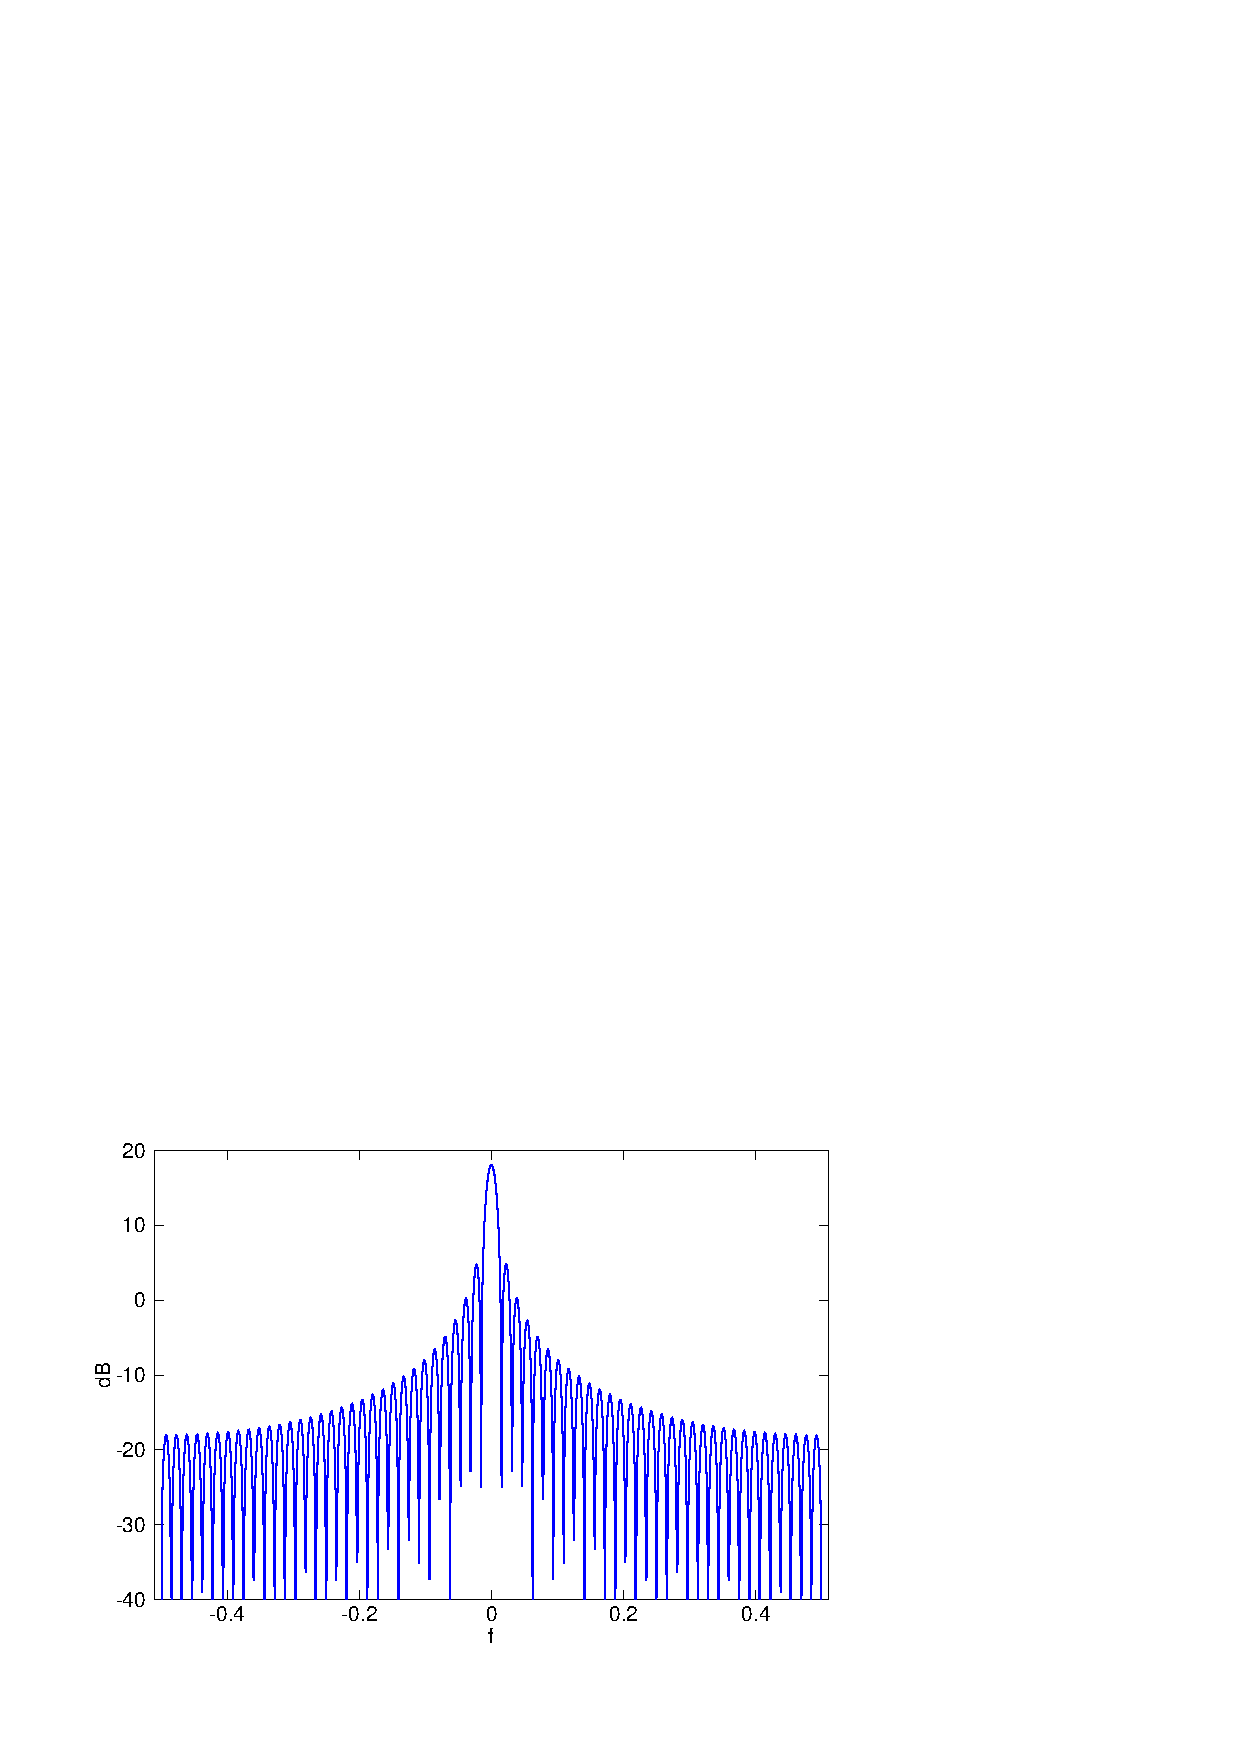
\includegraphics[width=4.5in]{pics/fejer64.pdf}
    \caption[Fej\'er's kernel]{Fej\'er's kernel, N=64 \label{fig:fejer}}
\end{figure}

\subsection{Data Tapers \label{sec:tapers}}

It can be shown that if the data is first windowed (or tapered) by a function, $\tilde{x}(t)=h(t)x(t)$, then the periodogram of this windowed function is related to the true spectrum:
\begin{align}
    \hat{S}^{(d)}(f) & = \frac{1}{T}\|\mathcal{F}(\tilde{x})(f)\|^2, & E\left[\hat{S}^{(d)}(f)\right] & = \int_{-1/2}^{1/2}H(f-f^\prime)S(f^\prime)df^\prime,
\end{align}
where $H=\|\mathcal{F}(h)\|^2$.  $\hat{S}^{(d)}$ is what Percival and Walden \cite{percival:multitaper} refer to as a direct spectral estimator\index{direct spectral estimator}.  It remains to select an ideal taper, $h$.  Such an ideal taper must have finite support in time (in order to be applied to the finite measurements $x$), and would minimize the height of the side-lobes in the frequency domain.  

David Slepian at Bell Labs studied such concentration problems, and developed what are now known as the discrete prolate spheroidal sequences (DPSSs) \cite{slepian:seq}.  They are sometimes referred to as Slepian sequences in his honour.  The discrete version of the concentration problem is as follows:
\smallskip

\begin{problem}
    Given a finite number of points, $n$, and a normalized bandwidth, $W$, find the sequence with the maximum concentration of energy in the frequency range $[-W,W]$.  
\end{problem}
\smallskip

\noindent In other words, we seek a sequence $\{h\}$ that maximizes
\begin{align}
    \lambda = \alpha^2(h) = \dfrac{\int_{-W}^W \|\mathcal{F}(h)(f)\|^2df}{\int_{-1/2}^{1/2} \|\mathcal{F}(h)(f)\|^2 df}. \label{eq:conc}\index{discrete prolate spheroidal sequence (DPSS)!concentration problem}
\end{align}
This becomes an eigenvalue problem, where the eigenvalues correspond to concentrations of energy in $[-W,W]$\index{energy concentration|see{eigenvalues}}.  The first discrete prolate spheroidal sequence (DPSS) is the eigenvector corresponding to the largest eigenvalue\index{discrete prolate spheroidal sequence (DPSS)!definition}.  The second DPSS is the eigenvector corresponding to the next largest eigenvalue, etc\ldots\  By definition, these sequences are orthonormal.  Example sequences are plotted in Figure \ref{fig:dpss}.  The actual computation of the DPSSs is outlined in Section \ref{sec:dpsscalc}.

\begin{figure}
    \centering
    \includegraphics[width=4.5in]{pics/dpss64.pdf}
    \caption[Discrete prolate spheroidal sequences]{Discrete prolate spheroidal sequences, $n=64$, $nW=2$.  The first four sequences are plotted: \textcolor{blue!80!black}{$h_0$}, \textcolor{green!40!black}{$h_1$}, \textcolor{red!80!black}{$h_2$} and \textcolor{green!60!blue!90!black!90}{$h_3$}, which have corresponding energy concentrations 0.9999, 0.9976, 0.9596 and 0.7220. \label{fig:dpss}}
\end{figure}

The DPSSs are described by their length, $n$, and \emph{time-bandwidth product} $nW$\index{time-bandwidth product} (sometimes called time-half-bandwidth product). The normalized frequency $W$ is half the width of the main lobe for these sequences, which defines the resolution.  There is a trade-off between the width of the main lobe, and the height of the side-lobes: decreasing one increases the other.  Thus, reducing $W$ increases the resolution, but also increases the broad-band bias.  This is demonstrated in Figure \ref{fig:dpssnw}.  Compare the height of the side-lobes in this figure to that of the Fej\'er kernel.  Although the width of the main-lobe has increased, the side-lobes drop-off more rapidly and to much lower values (levelling at -50 dB for $nW=2$ and -100 dB for $nW=4$).  

It can be shown that the first $\lfloor2nW\rfloor$ sequences have energy concentrations near one.  After this index, the eigenvalues rapidly decrease to zero, meaning most of the energy is contained in the side-lobes.  Thus, only the first few DPSSs are useful in spectrum calculations.

\begin{figure}
    \centering
    \includegraphics[width=4.75in]{pics/dpss_nw64.pdf}
    \caption[Spectrum of DPSS$_0$]{Spectrum of $h_0$ for $n=64$, \textcolor{blue!80!black}{$nW=2$} and \textcolor{green!40!black}{$nW=4$}. \label{fig:dpssnw}}
\end{figure}

David Thomson, a colleague of Slepian's, was the first to apply these sequences to frequency estimation.  Using the first DPSS as a data taper, the resulting direct spectrum estimate is guaranteed to have low broad-band bias characteristics.  The cost of tapering is that some of the data is effectively thrown away.  By examining Figure \ref{fig:dpss}, it can be seen that $h_0$ places more emphasis on data points near the centre of the time-series, and discards data near the ends.  The higher sequences, however, place more and more emphasis on data near the end-points.  

Each taper can be used to produce a different spectrum estimate, placing emphasis on different data points:
\begin{align}
    \hat{S}_k(f)(f) & = \|\hat{J}_k(f)\|^2 = \|\mathcal{F}(h_kx)(f)\|^2, \quad k=0,\ldots,K-1, \label{eq:eigencoeffs}
\end{align}
where $K<\lfloor2nW\rfloor$.  Thomson refers to $\{J_k\}$ as the \emph{eigencoefficients}\index{eigencoefficient} of the sample, and $\{S_k\}$ as the \emph{eigenspectra}\index{eigenspectrum} \cite{thomson:multitaper}.  It can be shown that for orthogonal tapers (such as the Slepian Sequences), the individual eigenspectra are approximately pair-wise uncorrelated.  Therefore, they can be averaged together in order to produce a single estimate, reducing overall variance.  Other conventional methods for reducing variance, such as the use of Welch's overlapping-segments or lag-windows, result in a reduction in resolution and an increase in bias.  The multitaper approach does not suffer these drawbacks (at least, not to the same extent).

\subsection{The Multitaper Spectral Estimator}

A single estimate of the power spectral density function can be obtained by simply averaging the uncorrelated eigenspectra:
\begin{align}
    \hat{S}_1^{(mt)}(f) & = \frac{1}{K}\sum_{i=1}^K \hat{S}_k(f).\index{multitaper spectral estimator!equal weighting}
\end{align}
This is the basic multitaper method, where equal weight is placed on each eigenspectrum.  The general form allows any weights,
\begin{align}
    \hat{S}^{(mt)}(f) & = \sum_{i=1}^K w_k\hat{S}_k(f),\index{multitaper spectral estimator!general form}
\end{align}
where $\sum_kw_k = 1$.  How should the weights be chosen?  It is known that the first taper is the most concentrated in $[-W,W]$, meaning it has better broad-band bias characteristics.  The second taper is the next most concentrated, etc\ldots\ It can be shown that the best linear estimator is to weight by the eigenvalues \cite{thomson:lecture}:
\begin{align}
    w_k & = \dfrac{\lambda_k}{\sum_{i=0}^{K-1}\lambda_i},  & \hat{S}_\lambda^{(mt)}(f)  & = \dfrac{1}{\sum_{i=0}^{K-1}\lambda_i}\sum_{i=0}^{K-1} \lambda_k \hat{S}_k(f),\index{multitaper spectral estimator!eigenvalue weighting}
\end{align}
where $\lambda_k=\alpha^2(h_k)$, the energy concentration for the $k$th DPSS.  For $K\leq\lfloor2nW\rfloor-1$, this estimate is approximately equivalent to $\hat{S}_1^{(mt)}$.  

A more sophisticated averaging scheme can be constructed by first estimating the bias at each frequency, then adjusting the weights to try to minimize this quantity.  It can be shown that in order to minimize the broad-band bias in the mean-square sense, the weights should satisfy
\begin{align}
    w_k(f) & = \dfrac{\lambda_k b_k^2(f)}{\sum_{i=0}^{K-1}\lambda_ib_i^2(f)}, & b_k(f) &= \dfrac{S(f)}{\lambda_kS(f)+(1-\lambda_k)\sigma^2},  \index{adaptive weights} \label{eq:adaptweights}
\end{align}
where $\sigma^2$ is the variance of the process \cite{percival:multitaper}.  Note that these weights are frequency-dependent, and also depend on the true spectrum.  Of course, the true spectrum is unknown, so the weights must be solved iteratively: begin with an initial estimate of the spectrum, then estimate a new set of weights.  These are used to update the spectrum estimate, which can be used to find new weights, etc\ldots\ The method quickly converges after a few iterations.  The result is that when the spectrum is deemed to be mostly dominated by bias, higher weight is placed on the first eigenspectrum (which has the best bias characteristics).  When the spectrum contains significant frequency content, the eigenspectra are weighted more equally, minimizing variance and maximizing the degrees of freedom.  This is known as \emph{adaptive weighting}, and the final spectrum is given by:
\begin{align}
    \hat{S}_a^{(mt)}(f) & = \dfrac{\sum_{k=0}^{K-1} b_k^2(f)\lambda_k \hat{S}_k(f)}{\sum_{k=0}^{K-1} b_k^2(f)\lambda_k}. \label{eq:adaptspec} \index{multitaper spectral estimator!adaptive weighting}
\end{align}

\subsection{Removal of the Mean \label{sec:removemean}}

It is common practice to remove an estimate of the mean-value from a time-series prior to tapering and computing the spectrum.  Constant trends introduce a strong local bias, making it difficult to estimate other low-frequency content, as well as a broad-band bias, which can hide low-power frequencies.  Also, non-zero means are rather easy to detect and remove.

\begin{figure}[!tb]
    \centering
    \includegraphics[width=4.75in]{pics/mean_remove128.pdf}
    \caption[Removing weighted means to reduce bias]{Multitaper spectrum estimate of $x(t)=3+\sin(2\pi0.015t)$, with $n=128$, $nW=2$, $K=3$.  In the \textcolor{blue!80!black}{first} estimate, the weighted means are removed; in the \textcolor{green!40!black}{second}, they are not. \label{fig:mt_mean}}
\end{figure}

Instead of estimating the mean in the usual way, consider the following weighted average:
\begin{align*}
    \hat{\mu} & = \dfrac{\sum_{t=0}^{n-1} h(t)x(t)}{\sum_{t=0}^{n-1} h(t)}.\index{weighted mean}
\end{align*}
As $n$ becomes large, it is easily shown that $\hat{\mu}$ (when defined) converges to the true mean.  If this weighted mean is removed from the data, the zero-frequency direct estimate becomes
\begin{align*}
    \hat{S}^{(d)}(0) & = \left\|\sum_{t=0}^{n-1}h(t)\left(x(t)-\hat{\mu}\right)\right\|^2\\
& = \left\|\sum_{t=0}^{n-1}h(t)x(t) - \left(\sum_{t=0}^{n-1}h(t)\right)\dfrac{\sum_{t=0}^{n-1} h(t)x(t)}{\sum_{t=0}^{n-1} h(t)} \right\|^2 = 0.\index{weighted mean!removal of}
\end{align*}
Since $\hat{S}^{(d)}(0)$ is forced to zero, it will not impact the estimate at any other frequency.  Any constant trend will be completely removed.  Unfortunately, odd tapers (like odd-numbered DPSSs) sum to zero, so the weighted mean is undefined.  However, any constant times an odd function is still an odd function, which always has a zero mean.  Therefore, subtracting any constant term from the data when an odd taper is used will not affect the direct spectrum estimate evaluated at $f=0$.  So, for odd tapers, it doesn't matter if the data is shifted by a constant, the resulting zero-frequency estimate will always be
\begin{align*}
    \hat{S}^{(d)}(0) & = \left\|\sum_{t=0}^{n-1}h_{\text{odd}}(t)x(t)\right\|^2.
\end{align*}
For numerical considerations, however, it is advised that the standard mean, $\bar{\mu}=\sum_t x(t)/n$, be removed.

The effect of removing the weighted means is shown in Figure \ref{fig:mt_mean}.  Notice that when the means are removed, the two peaks at $f=-0.015$ and $f=0.015$ are clearly discernible.  When the mean is not removed, they are not.  Also, notice the large difference in the level of broad-band bias (about 25 dB).

\subsection{Confidence Intervals} \index{confidence interval|(}

In order to have some level of confidence in the computed power spectral density, one must examine the statistical properties of the estimate.  For a real-valued stationary time-series and $n$ `large enough', direct spectrum estimates are approximately distributed as follows:
\begin{align}
    \hat{S}^{(d)}(f) & \sim \begin{cases}
                                S(f) \chi^2_1, & \text{for }f \in B_\delta(0) \cup B_\delta(\pm1/2)\\
                                \frac{1}{2} S(f) \chi^2_2, & \text{for } \delta < |f| < \tfrac{1}{2}-\delta,
                            \end{cases}\index{direct spectral estimator!distribution of}
\end{align}
where $\delta$ is related to the resolution of the estimate (Rayleigh resolution for the periodogram, $W$ for the eigenspectra), and $B_\delta(x)=(x-\delta, x+\delta)$.   Also, for large $n$, the estimates at two frequencies separated by the resolution are approximately uncorrelated:
\begin{align}
    \text{cov}\left\{\hat{S}^{(d)}(f_1), \hat{S}^{(d)}(f_2)\right\} & = 0, \quad \delta < f_1,f_2 < \tfrac{1}{2}-\delta,\;\; |f_1-f_2|>2\delta.
\end{align}
These statistics are asymptotic as $n\to\infty$, but are still useful in practice.

For the multitaper estimate, several uncorrelated direct spectrum estimates are averaged.  This means that $\hat{S}^{(mt)}$ is distributed as the weighted sum of uncorrelated chi-squared distributions, which is also approximately chi-squared distributed.  Letting $\hat{S}^{(mt)}=\sum_k w_k\hat{S}_k$, the approximate distribution is
\begin{align}
    \hat{S}^{(mt)}(f) & \sim \frac{1}{\nu} S(f) \chi^2_\nu,\index{multitaper spectral estimator!distribution of}\\
\text{where }\quad \nu & = \begin{cases}
                        \phantom{2}\left(\sum_{k=0}^{K-1} w_k^2\right)^{-1} & \text{for }f \in B_\delta(0) \cup B_\delta(\pm1/2)\\
                        2\left(\sum_{k=0}^{K-1} w_k^2\right)^{-1} & \text{for } \delta < |f| < \tfrac{1}{2}-\delta.
                   \end{cases}  \label{eq:dof}\index{degrees of freedom}
\end{align}
Here, $\nu$ is the equivalent degrees of freedom in the estimate.  The larger $\nu$ is, the smaller the variance.  The degrees of freedom are maximized when equal weights are used ($w_k=1/K$, $\nu=2K$), demonstrating the trade-off between variance and bias.  Note that for linear weighting schemes (like equal or eigenvalue weighting), $\nu$ is constant across frequencies (apart from near zero and one-half).  For adaptive weighting, $\nu$ is frequency-dependent.

Given the approximate statistical distribution of the estimate, a confidence interval can be constructed such that
\begin{align*}
    P\left[S(f) \in \mathcal{C}(p)(f)\right]=p.\index{confidence interval}
\end{align*}
At each frequency, the $p=(1-2q)\times100\%$ confidence interval is given by
\begin{align}
    \mathcal{C}(p)(f)=\left[\dfrac{\nu}{Q_\nu(1-q)}\hat{S}(f)\;,\;\dfrac{\nu}{Q_\nu(q)}\hat{S}(f)\right],
\end{align}
where $Q_\nu(q)$ is the quantile for a $\chi^2_\nu$ distribution: $P\left[\chi^2_\nu\leq Q_\nu(q)\right]=q$.  The width of this interval gives an indication of the estimate's accuracy.

\begin{figure}
    \centering
    \includegraphics[width=4.75in]{pics/conf_int256.pdf}
    \caption[Confidence interval example]{Multitaper \textcolor{blue!80!black}{spectrum estimate} of $x(t)=\sin(2\pi0.2t)+\cos(2\pi0.4t) + \eta(t)$, with $n=256$, $nW=2$, $K=3$, $\sigma_\eta=0.5$ and eigenvalue weighting.  The 95\% confidence interval is also plotted. \label{fig:conf_int}}
\end{figure}

The analysis for complex-valued time-series' is slightly easier since no special case is required for $f$ near zero or one-half.  The distribution and confidence interval are the same as the $f\in(\delta, \tfrac{1}{2}-\delta)$ case \cite{percival:multitaper}.
\index{confidence interval|)}

\subsection{F-test for Significant Frequencies \label{sec:ftest}} \index{F-test|(}

One of the main advantages of Thomson's multitaper analysis is that it lends itself well to a simple test for statistically significant line frequencies.  The estimated eigencoefficient at frequency $f$ can be modelled as
\begin{align}
    \hat{J}_k(f) & = J_k(f) + \epsilon_k, \quad \epsilon_k=\mathcal{F}(\eta_k)(f),
\end{align}
where $\eta_k$ is a noise parameter, assumed to be a white complex Gaussian random variable.  If there is no significant energy at $f$, then the true eigencoefficient will satisfy $\|J_k(f)\|^2=0$.  Otherwise, $\|J_k(f)\|^2$ is expected to be much greater than zero.  Under the assumption that $f$ is not significant, we can construct an estimate of the spectrum which depends on the noise parameter, $\eta_k$.  This will be approximately chi-squared distributed, since $\|\mathcal{F}(\eta_k)(f)\|^2$ is.  We can then check this against the calculated spectrum, which is also chi-squared distributed.  The ratio of the two is F-distributed, allowing the use of the F-test\index{F-test}.  The null-hypothesis is that $f$ is not a significant, meaning the spectrum can be explained by noise.  If the test fails, then $\hat{J}_k(f)$ cannot be explained by just noise.

The following is an adapted version of Percival and Walden's F-test description.  In \cite{percival:multitaper}, all eigencoefficients are equally weighted in the construction of the F-distribution.  However, for eigenvalue and adaptive weighting, it is known that some eigencoefficients have more of an impact on the estimated spectrum than others.  The effect of including different weights is considered here.

It can be shown that
\begin{align}
    \hat{J}_k(f) & \approx C(f) H_k(0)+\epsilon_k, \label{eq:eigcoeffapprox}
\end{align}
where $C$ is the unknown Fourier coefficient of $x$ at $f$, and $H_k=\mathcal{F}(h_k)$.  To proceed, $C$ must be estimated from the computed eigencoefficients.  If the $k$th eigenspectrum affects the spectrum estimate with weight $w_k$, then the $k$th eigencoefficient should affect the Fourier coefficient estimate with a weight $\propto\sqrt{w_k}$.  An estimate of $C$ from Equation \eqref{eq:eigcoeffapprox} is therefore given by
\begin{align}
    \hat{C}(f) & = \dfrac{\sum_{k=0}^{K-1}\sqrt{w_k(f)}H_k(0)\hat{J}_k(f)}{\sum_{k=0}^{K-1}\sqrt{w_k(f)}H^2_k(0)}.
\end{align}
This coefficient is a complex Gaussian random variable with mean $C(f)$ and variance
\begin{align}
    \sigma_{\hat{C}}^2 & = \sigma_\epsilon^2 \left(\sum_{k=0}^{K-1}\sqrt{w_k(f)}H^2_k(0)\right)^{-1}.
\end{align}
The noise power can be estimated by
\begin{align}
    \hat{\sigma}^2_\epsilon & = \sum_{k=0}^{K-1}w_k\|\hat{J}_k - \hat{C}H_k(0)\|^2. 
\end{align}
This is the expected power at $f$ under the null hypothesis.  Rescaling this random variable leads to
\begin{align}
    \left[\dfrac{\nu}{\sigma_\epsilon^2}\right]\hat{\sigma}^2_\epsilon & \sim \chi^2_{\nu-2}, \label{eq:chi1}
\end{align}
where $\nu$ is the degrees of freedom of $\hat{S}^{(mt)}$ at $f$.  Two degrees of freedom were lost because of the estimation of the parameter $C$, which is complex-valued.

Another approximate power at $f$ is given by $\|\hat{C}(f)\|^2$.  Under the null-hypothesis, $C(f)=0$, so $\hat{C}$ follows a complex Gaussian random variable with zero mean.  Thus, it's squared norm follows a scaled chi-squared distribution:
\begin{align}
    \left[\dfrac{2 \left(\sum_{k=0}^{K-1} \sqrt{w_k}H_k(0)^2\right)^2 }{ \sigma_\epsilon^2 \sum_{k=0}^{K-1} w_k H_k(0)^2}\right]\|\hat{C}\|^2 & \sim \chi_2^2. \label{eq:chi2}
\end{align}
The ratio of the two random variables described in Equations \eqref{eq:chi1} and \eqref{eq:chi2}, divided by their respective degrees of freedom, is F-distributed:
\begin{align}
    \dfrac{\|\hat{C}\|^2\left(1-\sum_{k=0}^{K-1} w_k^2\right) \left(\sum_{k=0}^{K-1} \sqrt{w_k}H_k(0)^2\right)^2}{\hat{\sigma}_\epsilon^2\sum_{k=0}^{K-1} w_k H_k(0)^2} & \sim F_{2,\nu-2} \label{eq:Fdist}\index{F-test}
\end{align}
If $C\neq 0$, then this F-statistic should report a value that exceeds some high percentage point of $F_{2,\nu-2}$, say $p\times 100\%$.  In such a case, we say that the null-hypothesis is rejected at the $(1-p)\times100\%$ level.

The upper $(1-\alpha)\times100\%$ percentage point of an $F_{2,\beta}$ distribution is easily computed:
\begin{align}
    F_u & = \dfrac{\beta\left(1-\alpha^{2/\beta}\right)}{2\alpha^{2/\beta}}. \index{F-test}
\end{align}
This threshold can grow exceedingly large if $\beta=\nu-2$ is small.  Recall that for equal weights, $w_k=1/K$ and $\nu=2K$.  However, in adaptive weighting, if the spectrum at a particular frequency is dominated by bias, then the weights are adjusted to heavily favour $\hat{S}_0$.  In the extreme case where $w_0\to1^{-}$, we have 
\begin{align*}
    \nu\to2^{+}\implies\beta\to0^{+}\implies 2/\beta\to\infty.
\end{align*}
Since $\alpha < 1$,
\begin{align*}
    \lim_{w_0\to1^{-}} \alpha^{2/\beta} = 0 \quad \implies \quad \lim_{w_0\to1^{-}} F_u = \infty.
\end{align*}
Thus, in adaptive weighting, the upper threshold for the F-test can grow infinitely high.  In this situation, however, a frequency heavily dominated by broad-band bias is not expected to be significant.  Therefore, the F-test for significant frequencies still behaves as expected.  In order to avoid the issue of an infinite threshold, the F-test can be performed for a linear weighting scheme.

\begin{figure}
    \centering
    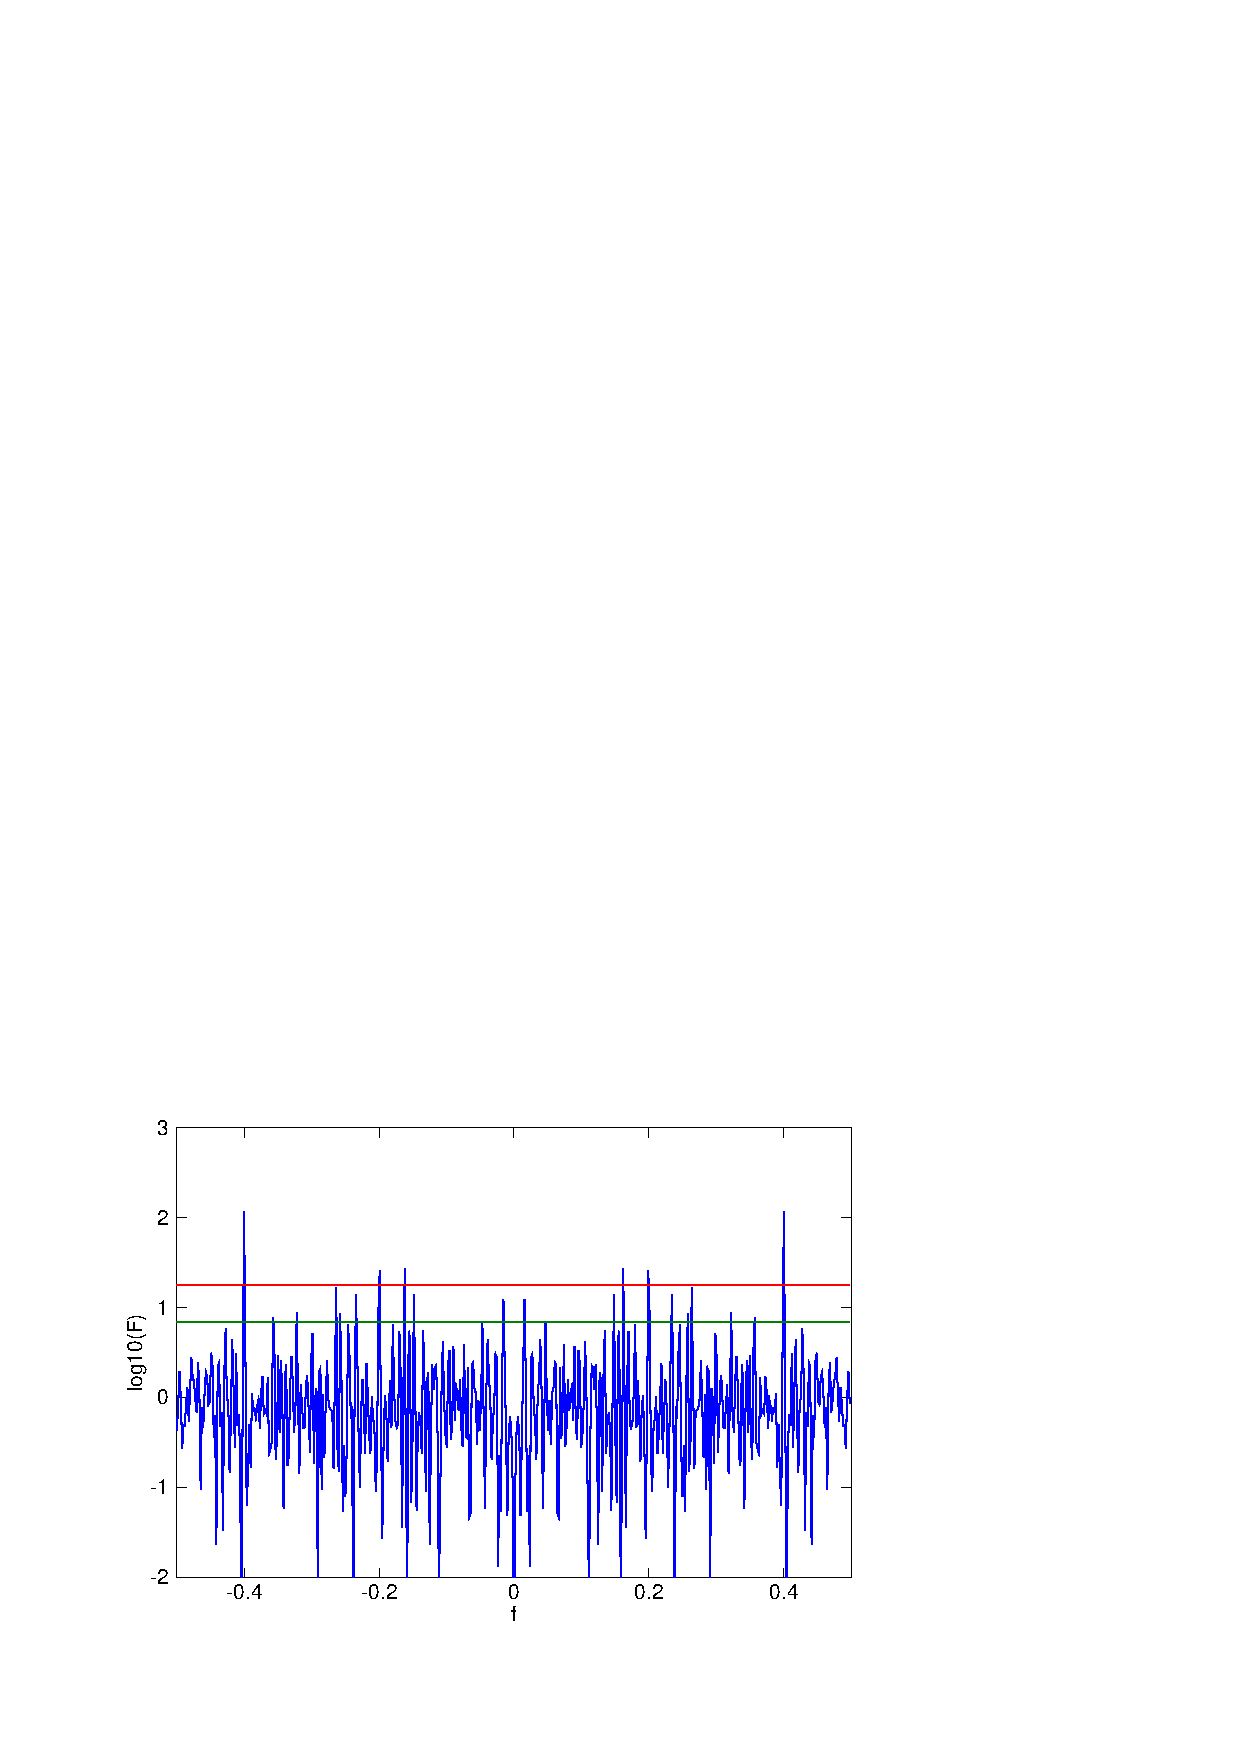
\includegraphics[width=4.75in]{pics/Fstat1_256.pdf}\\ 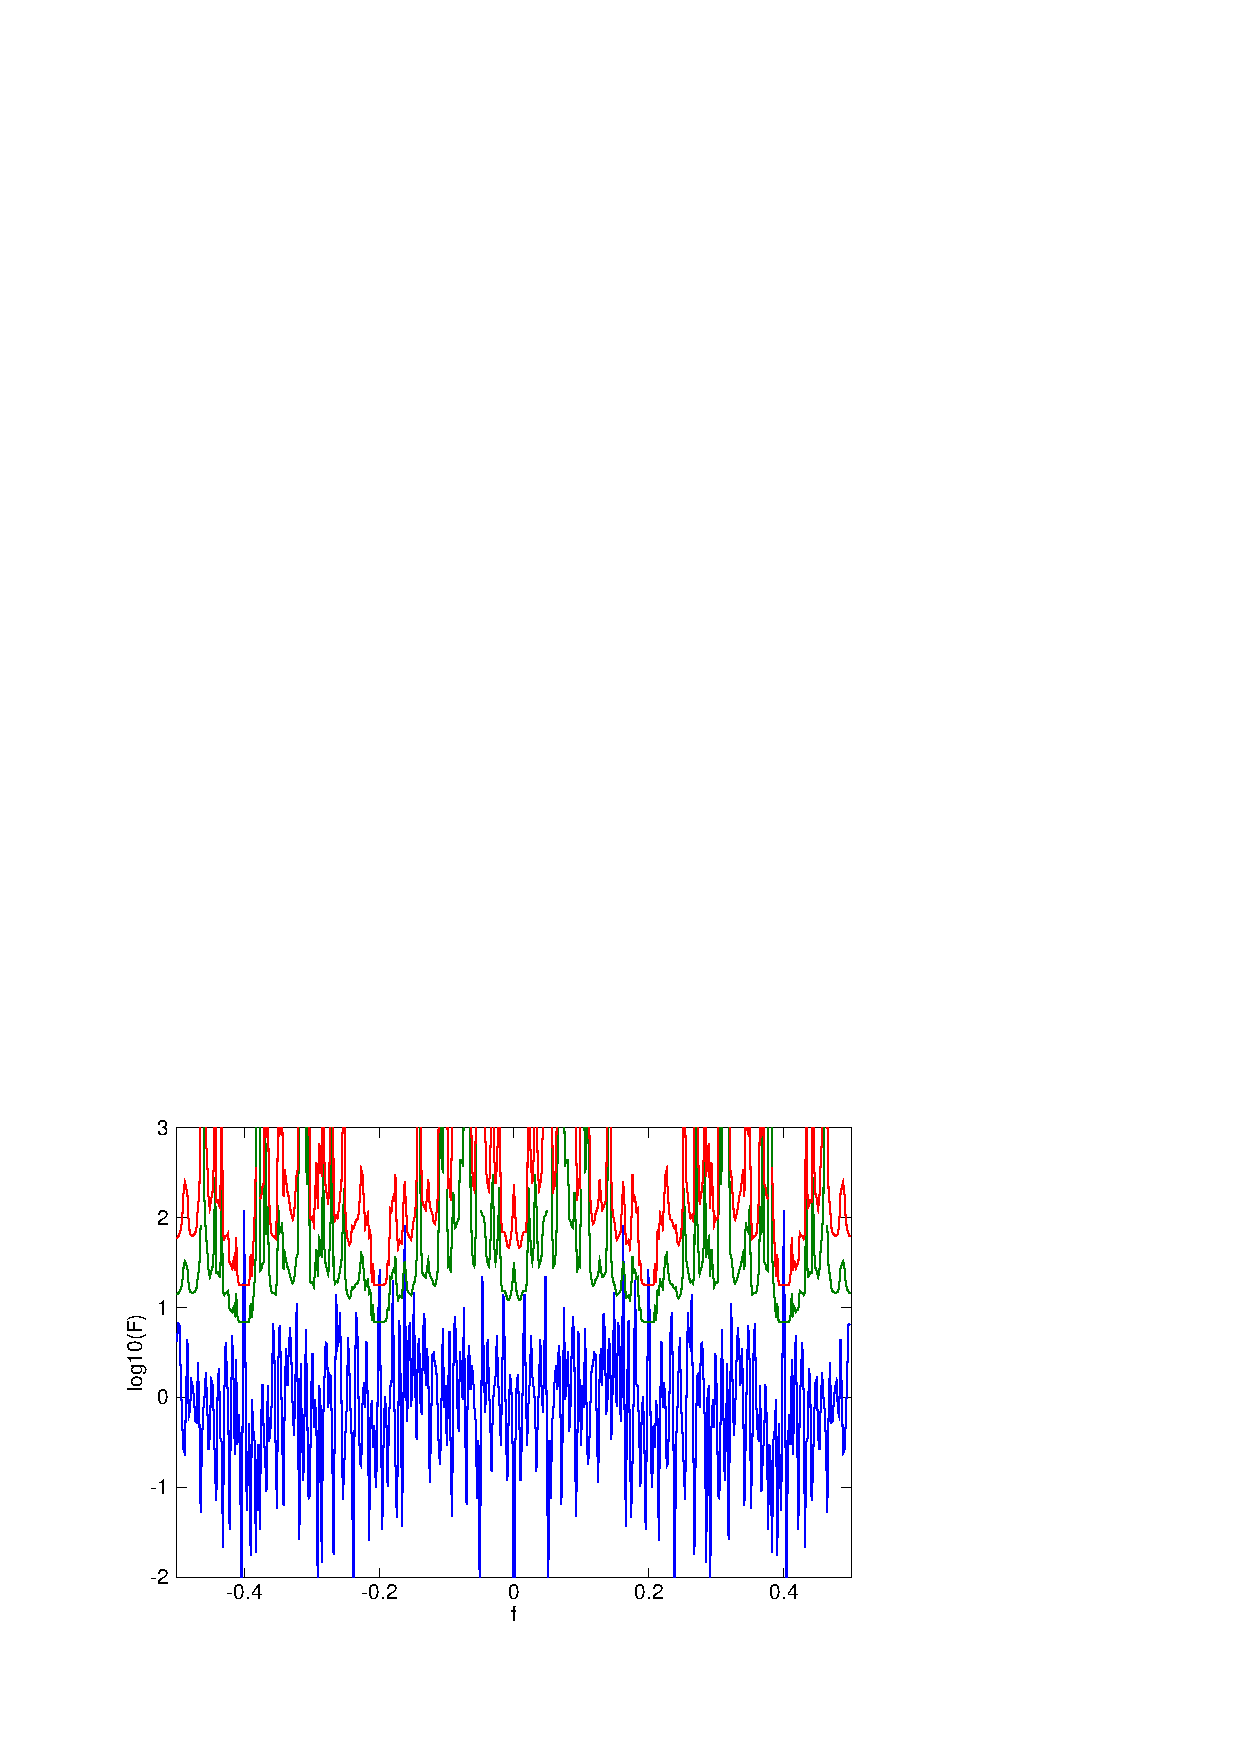
\includegraphics[width=4.75in]{pics/Fstat2_256.pdf}\\
    \caption[F-test example]{F-test at the \textcolor{green!40!black}{$p_1=95\%$} and \textcolor{red!80!black}{$p_2=99\%$} significance levels for $x(t)=\sin(2\pi0.2t)+\cos(2\pi0.4t) + \eta(t)$, where $n=256$, $nW=2$, $K=3$, and $\sigma_\eta=0.1$. The top results are eigenvalue weighted, and the bottom adaptive.\label{fig:f_stat}}
\end{figure}

For equal and eigenvalue weights, the number of degrees of freedom is constant across all frequencies.  This means $F_u$ is also constant.  For adapted weights, $F_u$ is frequency dependent, which can make a visual interpretation of the F-test more difficult.  Examples of F-tests are shown in Figure \ref{fig:f_stat}.  Notice that when adaptive weighting is used, the threshold dips down at the four frequencies $f=\pm 0.2, \pm0.4$.  This is due to the increase in degrees of freedom at these frequencies.  At the 95\%  significance level, the adaptively-weighted F-test only gives false positives at $\pm 0.16$Hz, whereas the eigenvalue-weighted F-test has 18 false positives.  At the 99\% significance level, the adaptively-weighted F-test finds only the four significant frequencies, while the eigen-value weighted one still has false positives at $\pm 0.16$Hz.

One final note: if $w_k$ is replaced with $1/K$ in all the equations in this section, the results from Percival and Walden are recovered.
\index{F-test|)}

\pagebreak

\subsection{Computing the DPSSs \label{sec:dpsscalc}}

As described in Section \ref{sec:tapers}, the discrete prolate spheroidal sequences have a fixed length $n$ and maximize the concentration problem
\begin{align*}
    \lambda = \alpha^2(h) = \dfrac{\int_{-W}^W \|\mathcal{F}(h)(f)\|^2df}{\int_{-1/2}^{1/2} \|\mathcal{F}(h)(f)\|^2 df}. \tag{\ref{eq:conc}}
\end{align*}
By applying the discrete Fourier transform, Equation \eqref{eq:conc} can be re-written in a discrete form:
\begin{align*}
    \lambda & = \left(\sum_{t=0}^{n-1}\|h(t)\|^2\right)^{-1}\sum_{t=0}^{n-1}\sum_{\tau=0}^{n-1} h(t)h(\tau)\dfrac{\sin\left[2\pi W(t-\tau)\right]}{\pi(t-\tau)}.
\end{align*}
The sequence $\{h(t)\}$ that maximizes this quantity satisfies
\begin{align}
    \sum_{\tau=0}^{n-1} \dfrac{\sin\left[2\pi W(t-\tau)\right]}{\pi(t-\tau)} h(\tau) & = \lambda h(t), \quad t=0,1,\ldots,n-1,
\end{align}
which is readily seen as the eigenvalue problem:
\begin{align}
    A h & = \lambda h, \quad \text{where }A_{ij} = \dfrac{\sin\left[2\pi W(i-j)\right]}{\pi(i-j)}. \label{eq:eigen}\index{discrete prolate spheroidal sequence (DPSS)!eigenvalue problem}\index{eigenvalues}\index{eigenvectors}
\end{align}
This produces $n$ orthonormal sequences, with eigenvalues that correspond to their concentration of energy in the normalized frequency range $[-W,W]$.  

Solving Equation \eqref{eq:eigen} can be difficult since the eigenvalues are so closely bunched together: the first $\lfloor 2nW \rfloor-1$ eigenvalues are very close to one, and the last $n-\lfloor 2nW \rfloor-1$ are clustered near zero.  This makes the problem numerically ill-conditioned.  Slepian \cite{slepian:seq} noticed that the eigenvectors satisfy a second set of equations:
\begin{align}
    \begin{gathered}
        u(t-1) h(t-1) + d(t) h(t) + u(t) h(t+1) = \theta h(t), \quad t=0,1,\ldots,n-1,\\
        u(t) = \dfrac{(t+1)(n-t-1)}{2}, \quad d(t)  = \left(\dfrac{n-1-2t}{2}\right)^2\cos(2\pi W).
    \end{gathered}\label{eq:tridiag}\index{discrete prolate spheroidal sequence (DPSS)!tridiagonal formulation}
\end{align}
Not only is this new eigenvalue problem much simpler to solve due to its symmetric tridiagonal structure, but the new eigenvalues ($\theta_k$) have a much better spread \cite{thomson:lecture}.  Thus, the discrete prolate spheroidal sequences can be computed using the system in Equation \ref{eq:tridiag}, and the energy concentrations recovered by then solving for $\lambda$ using Equation \ref{eq:eigen}:
\begin{align}
    \lambda & = \dfrac{h^\text{T}Ah}{\|h\|^2}. \label{eq:eigenvalue}
\end{align}


There are other ways of solving for the DPSSs, including Gaussian quadrature techniques \cite{thomson:multitaper}, and inverse iteration methods \cite{percival:multitaper}.  However, the tridiagonal matrix method is incredibly fast, stable, and accurate, and is the one recommended by Thomson \cite{thomson:lecture}.

\subsubsection{Even-Odd Splitting \label{sec:splitting}}

The doubly-symmetric nature of the systems in \eqref{eq:eigen} and \eqref{eq:tridiag} cause the even eigenvectors $\{h_0,h_2,\ldots\}$ to be even functions about their centre, and the odd eigenvectors $\{h_1,h_3,\ldots\}$ to be odd functions.  This means that only the first $\lceil n/2 \rceil$ elements of the vectors need to be calculated.  This allows the problem to be split in two: one for even sequences, where $h(i)=h(n-1-i)$, and one for odd, $h(i)=-h(n-1-i)$ \cite{slepian:compute}.  The tridiagonal matrices for the subproblems are described as follows:\index{discrete prolate spheroidal sequence (DPSS)!even-odd splitting}
\begin{align*}
       & \qquad\text{Even}\ n &  &\qquad\text{Odd}\ n\\[0.3em]
    d_e(i) & = d(i),\quad i=0,\ldots,\tfrac{n}{2}-2 &               d_e(i) & = d(i),\quad i=0,\ldots,\tfrac{n+1}{2}\\
    d_e(\tfrac{n}{2}-1) & = d(\tfrac{n}{2}-1)+u(\tfrac{n}{2}-1) &   u_e(i) & = u(i), \quad i=0,\ldots,\tfrac{n-3}{2}\\
    u_e(i) & = u(i), \quad i=0,\ldots,\tfrac{n}{2}-2 &              u_e(\tfrac{n-1}{2}) & = \sqrt{2}\,u(\tfrac{n-1}{2})\\
    \\
    d_o(i) & = d(i),\quad i=0,\ldots,\tfrac{n}{2}-2 &               d_o(i) & = d(i),\quad i=0,\ldots,\tfrac{n-1}{2}\\
    d_o(\tfrac{n}{2}-1) & = d(\tfrac{n}{2}-1)-u(\tfrac{n}{2}-1) &   u_o(i) & = u(i),\quad i=0,\ldots,\tfrac{n-3}{2}\\
    u_o(i) & = u(i), \quad i=0,\ldots,\tfrac{n}{2}-2
\end{align*}
where subscripts $e$ and $o$ represent entries for the even and odd subproblems, respectively.  Note that for $n$ odd, a factor $\sqrt{2}$ is necessary to maintain symmetry.  As a result, the centre value must be rescaled when constructing the final sequences: $h(\tfrac{n-1}{2})=\sqrt{2}\,h_e(\tfrac{n-1}{2})$.

Splitting into even and odd subproblems reduces memory requirements, increases computation speed, and also increases the stability of the algorithm: the eigenvalues of the new systems are now separated twice as far as the original, allowing for improvements in accuracy \cite{thomson:lecture}.
\clearpage

\newsection{The Package \label{sec:package}}
The \code{mtpsd} library is a combination of two projects: one for computing the discrete prolate spheroidal sequences, and one for computing multitaper spectrum estimates.  It is possible to compile two static libraries:
\smallskip

\begin{tabular}{lp{\textwidth-25ex}}
    \texttt{libdpss.a}\index{libdpss@\texttt{libdpss}} & Provides methods for computing DPSSs.\\
    & Dependencies: \texttt{libfftw3}.\\
    \texttt{libmtpsd.a}\index{libmtpsd@\texttt{libmtpsd}} & Provides methods for computing all multitaper estimates and properties described in Section \ref{sec:theory}, as well as for computing the DPSSs (i.e.~it \emph{includes} \texttt{libdpss.a}).\\
    & Dependencies: \texttt{liblapack}, \texttt{libfftw3}.
\end{tabular}
\smallskip

\noindent The two Octave extensions, \texttt{dpss.oct} and \texttt{mtpsd.oct}, provide an interface to the library.  They depend on the Octave \texttt{mkoctfile} utility.  The command-line application, \texttt{dpss}, uses the \texttt{dpss} library to compute DPSSs, and prints the results to \code{stdout}.

\subsection{Compiling}

Compiling the libraries is most easily accomplished with the GNU make utility.  The provided Makefile should work as-is for most Unix-based systems.
\smallskip

\noindent \begin{tabular}{@{\hspace*{4ex}}p{17ex}@{\hspace*{3ex}}p{\textwidth-28ex}@{\hspace*{4ex}}}
    \texttt{make [all]} & builds the two static libraries: \\
                        & \hspace*{4ex}\texttt{lib/libdpss.a}, \texttt{lib/libdpss.a}; \\
                        & the two octave extensions: \\
                        & \hspace*{4ex}\texttt{bin/dpss.oct}, \texttt{bin/mtpsd.oct}; \\
                        & and the command-line application:\\
                        & \hspace*{4ex}\texttt{bin/dpss}.\\
    \texttt{make lib} & builds \texttt{lib/libdpss.a} and \texttt{lib/libdpss.a}.\\
    \texttt{make oct} & builds \texttt{bin/dpss.oct} and \texttt{bin/mtpsd.oct}.\\
    \texttt{make nooct} & builds \texttt{lib/libdpss.a}, \texttt{lib/libdpss.a}, and \texttt{bin/dpss}.
\end{tabular}
\smallskip

\noindent There is no `install' directive.  All binaries and Octave extensions are placed in the local \texttt{bin/} directory, C++ libraries in \texttt{lib/}, and header files in \texttt{include/}.  See the Makefile for more building options.

For windows, you will need to edit the Makefile to point to the correct compiler.  If you are building the Octave extensions, that compiler must be compatible with your version of Octave.  For example, I have MinGW64 installed, but Octave provided by the \href{http://sourceforge.net/projects/octave/files/Octave_Windows\%20-\%20MinGW/Octave\%203.2.4\%20for\%20Windows\%20MinGW32\%20Installer/}{Octave Windows installer} was compiled with MinGW32.  I had to set:
\begin{itemize}
    \item[-] \texttt{CC=mingw32-g++-4.4.0-dw2.exe},\\
        the compiler provided by the Octave installation.
    \item[-] \texttt{MINGW\_PATH=/d/local/octave/mingw32},\\
        Octave's MinGW path, so the compiler can find the right libraries and executables.
    \item[-] \texttt{LIB\_PATH=/d/local/octave/lib},\\
        the path with Octave's versions of the LAPACK and FFTW3 libraries.
\end{itemize}
These parameters are near the top of the Makefile.

\subsection{Linking}

If you are using the GNU gcc compiler, use the \texttt{-static} option and link using \texttt{-lmtpsd}\index{libmtpsd@\texttt{libmtpsd}} (or \texttt{-ldpss}\index{libdpss@\texttt{libdpss}} for just that component).  You must also link to \texttt{liblapack} and \texttt{libfftw3}.  For example,
\begin{verbatim}
    gcc -static main.cpp -lmtpsd -llapack -lfftw3 -o my_prog
\end{verbatim}
will create the binary \texttt{my\_prog} from \texttt{main.cpp}.  Make sure the libraries can be found by the linker.  If you have not installed \texttt{libmtpsd} to a default search directory, you will need to pass the option \texttt{-L}\textit{/path/to/library}.  If your compiler complains about \code{dlamch_}, you must also link to the BLAS library (\texttt{-lblas}).  If you use the Fortran version of LAPACK, you may also need \texttt{-lgfortran}.

\subsection{Headers}

In order to use the C++ libraries, include the appropriate header file in your source code.  All headers are found in the \texttt{include/} directory.  The following is a short description of each of the available headers:

\begin{codelist}
    \item[mtpsd.h] contains the \code{mtpsd}\index{mtpsd class@\texttt  {mtpsd} class}\index{libmtpsd@\texttt{libmtpsd}} class and all methods required for computing the multitaper power spectral density of a time-series.
    \item[dpss.h] contains the \code{dpss}\index{dpss class@\texttt  {dpss} class}\index{libdpss@\texttt{libdpss}} class and all methods required for computing the discrete prolate spheroidal sequences.  This file is automatically included by \texttt{mtpsd.h}.
    \longitem{applied\_stats.h} contains procedures needed to compute quantiles of $\chi^2$ and Gaussian distributions.  This file is automatically included by \texttt{mtpsd.h}.
    \longitem{simple\_error.h} contains two error classes: one specific for LAPACK errors, and one general.  This file is automatically included by \texttt{dpss.h} and \texttt{mtpsd.h}.\index{ERR class@\texttt{ERR} class}\index{LAPACK_ERROR class@\texttt{LAPACK\_ERROR} class}
    \longitem{template\_math.h} contains some basic math/vector math operations, written using templates.  This file is automatically included by \texttt{dpss.h} and \texttt{mtpsd.h}.
\end{codelist}

\subsection{License}
\vspace*{0.5em}

\copyright~C.~Antonio S\'anchez 2010
\vspace*{0.5em}

\noindent \texttt{mtpsd} is free software: you can redistribute it and/or modify
it under the terms of the GNU General Public License as published by
the Free Software Foundation, either version 3 of the License, or
(at your option) any later version.
\vspace*{0.5em}

\noindent \texttt{mtpsd} is distributed in the hope that it will be useful,
but WITHOUT ANY WARRANTY; without even the implied warranty of
MERCHANTABILITY or FITNESS FOR A PARTICULAR PURPOSE.  See the
GNU General Public License for more details.
\vspace*{0.5em}

\noindent You should have received a copy of the GNU General Public License
along with \texttt{mtpsd}.  If not, see $<$\url{http://www.gnu.org/licenses/}$>$.
\newpage

\markboth{\textsc{Using the }\texttt{mtpsd}\textsc{ Library}}{}
\newsection{Using the \texttt{mtpsd} Library \label{sec:mtpsd}}
\markboth{\textsc{Using the }\texttt{mtpsd}\textsc{ Library}}{}
\index{mtpsd@\texttt{mtpsd}|(}There are two main ways to use the \texttt{mtpsd} library.  The first is through the use of an object.  The \code{mtpsd.h} header defines the \code{mtpsd} class, which can be used to compute any of the multitaper spectrum estimates and properties described in Section \ref{sec:theory}.  All of the internal variables are protected, so must be accessed through provided accessors.  One special accessor is defined, \code{mtpsd::pS()}, which returns a \code{const double} pointer to the protected spectrum array, allowing more direct access.  The class and its use are described in Section \ref{sec:basic}.

The second way to use the library allows for more control over memory and access to intermediate variables.  A set of functions are defined that accept and fill user-defined arrays.  For multi-dimensional arrays, row-major format is assumed.  This advanced use is covered in Section \ref{sec:advanced}.

\subsection{Basic Use: the \texttt{mtpsd} Class \label{sec:basic}}

Listing \ref{lst:basic} shows the most basic construction and use of an \code{mtpsd} object.  \index{mtpsd class@\texttt  {mtpsd} class|(}
\begin{lstlisting}[label=lst:basic,caption=Basic example of the \texttt{mtpsd} class]
#include "mtpsd.h"              /*@\lstomitnum@*/
...                             /*@\lstskipnum{8}@*/
{
    double *x;          // time series
    uint_t n;           // length(x), (unsigned int)
    double nW;          // time-bandwidth product   /*@\lstomitnum@*/
    ...                         /*@\lstomitnum\lstskipnum{7}@*/
    
    mtpsd<double> spectrum(x, n, nW);
    try{
        spectrum.compute();
    }
    catch(ERR e){
        printf("ERROR: %s\n", e.getmsg());   
    }                           /*@\lstomitnum@*/
    ...                         /*@\lstomitnum\lstskipnum{7}@*/
    
    printf("S=%f, f=%fHz \n", spectrum(i), spectrum.freq(i));    /*@\lstomitnum@*/
    ...                         /*@\lstskipnum{8}@*/
}
\end{lstlisting}\index{mtpsd class@\texttt  {mtpsd} class!compute@\texttt{compute()}}
\smallskip

\noindent In the example, the \code{spectrum} object contains all information pertaining to the multitaper estimate.  There are several things to note:
\begin{itemize}
    \item \code{mtpsd} is an \emph{template class}.  The library is configured to compile for types \code{double} and \code{fftw\_complex} (\code{double \_\_complex\_\_}).  This must correspond to the data type of the time-series \code{x}.
    \item The \code{compute()} method may throw an error of type \code{ERR}\index{ERR class@\texttt{ERR} class}.  This class is defined in \code{simple\_error.h} (see Section \ref{sec:simpleerr}).  The error class only has one property: an error message, accessible through \code{ERR::getmsg()}.
    \item All lengths and indices are of type \code{unsigned int}.  A short-form for this type, \code{uint\_t}\index{uint\_t@\texttt{uint\_t}}, is defined in the \code{mtpsd.h} header.
    \item This basic constructor assumes adaptive weighting, a sampling frequency of 1 Hz, and uses $K=\max\{\lfloor2nW\rfloor-1,2\}$ data tapers.
\end{itemize}
The desired spectrum information can be extracted through one of the object's accessors, which are described in Table \ref{tbl:mtpsdaccess}.  The public definition of the \code{mtpsd} class is given in Listing~\ref{lst:mtpsdclass}.
\smallskip

\index{mtpsd class@\texttt  {mtpsd} class!definition|(}
\begin{lstlisting}[label=lst:mtpsdclass,caption=The \texttt{mtpsd} class]
template <class T>
class mtpsd {
    // constructors/destructor
    mtpsd(T *data, uint_t n, double nW);                       /*@\label{lst:mtpsdconstruct1}@*/
    mtpsd(T *data, mtpsd_workspace work);                      /*@\label{lst:mtpsdconstruct2}@*/
    mtpsd(T *data, const double *tapers, const double *lambda, /*@\label{lst:mtpsdcustomtaper1}\lstomitnum\lstskipnum{99}@*/
             uint_t n, uint_t K);                              /*@\lstskipnum{-100}@*/
    mtpsd(T *data, const double *tapers, const double *lambda, /*@\label{lst:mtpsdcustomtaper2}\lstomitnum\lstskipnum{99}@*/
             mtpsd_workspace work);                            /*@\lstskipnum{-100}@*/
    ~mtpsd();
    
    // computation routine
    void compute();

    // accessors
    double operator()(uint_t i);           
    const double* pS();
    double operator()(uint_t k, uint_t i);
    fftw_complex eig_coeff(uint_t k, uint_t i); 
    double wt(uint_t k, uint_t i);       
    double freq(uint_t i);                
    double dof(uint_t i);                          
    double conf_int(uint_t i, CONF_BOUND side, double p); 
    double conf_factor(uint_t i, CONF_BOUND side, double p);
    double lambda(uint_t k);
    double taper(uint_t k, uint_t i);
    double F_stat(uint_t i);  
    double F_thresh(uint_t i, double p); 
    bool F_test(uint_t i, double p); 
    uint_t length();  
    uint_t size(int dim);
    mtpsd_workspace getinfo();
};
\end{lstlisting}\index{mtpsd class@\texttt  {mtpsd} class!compute@\texttt{compute()}}
\index{mtpsd class@\texttt  {mtpsd} class!definition|)}

\begin{table}
    \caption{ Description of \texttt{mtpsd}\index{mtpsd class@\texttt{mtpsd} class!accessors} accessors \label{tbl:mtpsdaccess} }
    \vspace*{-0.75em}
    
    \begin{tabular}{c}
        \hline\hline\\[-0.75em]
        \small
        \parbox{\textwidth-12pt}{
            \vspace*{-0.5em}
            \settowidth{\bodyindent}{\texttt{mtpsd\_workspace}}
            \begin{compactcodelist}
                \codeitem{double}{operator()(uint\_t i)}
                    Returns $\hat{S}(f_i)$, the power at the $i$th frequency (starting at $f_0=0$).
                \codeitem{const double*}{pS()}
                    Returns a pointer to the $\hat{S}$ array, so the data can be accessed directly.
                \codeitem{double}{operator()(uint\_t k, uint\_t i)}
                    Returns $\hat{S}_k(f_i)$, the $i$th value of eigenspectrum $k$. 
                \codeitem{fftw\_complex}{eig\_coeff(uint\_t k, uint\_t ii)}
                    Returns $\hat{J}_k(f_i)$, the $i$th value of eigencoefficient $k$.
                \codeitem{double}{wt(uint\_t k, uint\_t i)}
                    Returns the weight factor $w_k(f_i)$, where $\hat{S}=\sum w_k\hat{S}_k$.
                \codeitem{double}{freq(uint\_t i)}
                    Returns $f_i$, the $i$th frequency in Hz.  If the sampling frequency has not been specified, then $f$ is scaled to lie in the range $[0, 1]$.
                \codeitem{double}{dof(uint\_t i)}
                    Computes and returns $\nu(f_i)$ the equivalent degrees of freedom of $\hat{S}(f_i)$, assuming $\hat{S}\sim \frac{1}{\nu}S\chi^2_\nu$.
                \codeitem{double}{conf\_int(uint\_t i, CONF\_BOUND side, double p)}
                    Computes and returns the $p\times100\%$ confidence bound at frequency $f_i$, where \code{side} is either \code{UPPER} or \code{LOWER}.
                \codeitem{double}{conf\_factor(uint\_t i, CONF\_BOUND side, double p)}
                    Computes and returns either the lower or upper confidence factor $\nu/Q_\nu$.  The corresponding confidence bound is obtained by multiplying this factor by $\hat{S}$. Recall that for equal and eigenvalue weights, the confidence factor is independent of frequency.  
                \codeitem{double}{lambda(uint\_t k)}
                    Returns $\lambda_k$, the eigenvalue (energy concentration) of the $k$th taper.
                \codeitem {double}{taper(uint\_t k, uint\_t i)}
                    Returns $h_k(t_i)$, the $i$th value of the $k$th taper.
                \codeitem {double}{F\_stat(uint\_t i)}
                    Computes and returns the F-statistic at frequency $f_i$.
                \codeitem {double}{F\_thresh(uint\_t i, double p)}
                    Computes and returns the $p\times100\%$ threshold for the F-test at frequency $f_i$.  Recall that for equal or eigenvalue weights, this threshold is independent of frequency.
                \codeitem {bool}{F\_test(uint\_t i, double p)}
                    Computes the F-statistic and threshold, and returns \code{true} if the threshold is surpassed (i.e.~the frequency is deemed significant).
                \codeitem {uint\_t}{length()}
                    Returns $N$, the discrete length of the spectrum estimate (length of the frequency grid).
                \codeitem {uint\_t}{size(int dim)}
                    If \code{dim}=0, returns $N$.  If \code{dim}=1, returns $K$, the number of tapers used.
                \codeitem {mtpsd\_workspace}{getinfo()}
                    Returns a structure that contains all computation parameters used by the \code{mtpsd} class.
            \end{compactcodelist}
        }\\
        \hline
   \end{tabular}
\end{table}

\subsubsection{The \texttt{mtpsd\_workspace} Structure}

\index{mtpsd\_workspace@\texttt{mtpsd\_workspace}|(}For more control over the multitaper parameters, a special \code{mtpsd\_workspace} structure is available.  It's definition is outlined in Listing \ref{lst:mtpsdwork}.  The first six members of the structure specify the multitaper computation parameters.  The last two are set automatically by the \code{mtpsd} class.  The structure has two constructor methods to initialize default values: one takes no inputs, and the other accepts the data length and the time-bandwidth product.
\smallskip

\begin{lstlisting}[label=lst:mtpsdwork,caption=The \texttt{mtpsd\_workspace} structure]
enum WEIGHT_METHOD {ADAPT, EIGEN, EQUAL};
enum DATA_TYPE {REAL_DATA, COMPLEX_DATA};

struct mtpsd_workspace{
    // should be set manually                                [default]       
    uint_t n;                     // length of data             [0] 
    double nW;                    // time-bandwidth product     [1]
    WEIGHT_METHOD weight_method;  // type of weighting          [ADAPT]
    uint_t N;                     // length of the DFTs         [n]
    uint_t K;                     // number of tapers           [2nW-1]
    double Fs;                    // sampling frequency         [1]
    bool remove_mean;             // specifies if weighted      [true]
                                  //   means to be removed
    // set automatically
    DATA_TYPE dtype;              // data type (real or complex)
    uint_t nwk;                   // # independent wts per Sk

    // constructors
    mtpsd_workspace(): n(0), nW(1), weight_method(ADAPT), N(0),/*@\lstomitnum\lstskipnum{98}@*/
                   K(2), Fs(1), remove_mean(true),             /*@\lstomitnum@*/
                   dtype(REAL_DATA), nwk(0){ }                 /*@\lstskipnum{-100}@*/
    mtpsd_workspace(uint_t n_, double nW_):  n(n_), nW(nW_),   /*@\lstomitnum\lstskipnum{100}@*/
                   weight_method(ADAPT), N(n_), K(floor(2*nW_)-1),/*@\lstomitnum@*/
                   Fs(1), remove_mean(true), dtype(REAL_DATA),   /*@\lstomitnum@*/
                   nwk(n_){ }                                   /*@\lstskipnum{-103}@*/
};
\end{lstlisting}
\bigskip

Listing \ref{lst:workexample} shows an example of a workspace being used to initialize an \code{mtpsd} object.  If any of the supplied parameters are invalid, the \code{mtpsd} constructor will use the default values.  Alternatively, the \code{mtpsd\_workspace} can first be corrected by supplying it to the function:
\begin{lstplainblock}
void fix_workspace( mtpsd_workspace &myworkspace ).
\end{lstplainblock}\index{fix\_workspace@\texttt{fix\_workspace()}}
This will modify the invalid parameters in the supplied workspace directly.

\pagebreak

\begin{lstlisting}[label=lst:workexample,caption=Example using the \texttt{mtpsd\_workspace} ]
#include "mtpsd.h"              /*@\lstomitnum@*/
...                             /*@\lstskipnum{8}@*/
{
    fftw_complex *x;            // complex time series /*@\lstomitnum@*/
    ...                         /*@\lstskipnum{7}\lstomitnum@*/

    mtpsd_workspace params;

    params.n=100;               // x has 100 points
    params.nW=3.5;
    params.weight_method=EIGEN; // eigenvalue weighting
    params.N=512;               // 512-point spectrum
    params.K=10;                
    params.Fs=1000;             // 1 kHz
    params.remove_mean=false;   // mean not removed

    mtpsd spectrum<fftw_complex>(x, params);
    try{
        spectrum.compute();
    }
    catch(...){}                /*@\lstomitnum@*/
    ...                         /*@\lstskipnum{8}@*/
}
\end{lstlisting}
\index{mtpsd\_workspace@\texttt{mtpsd\_workspace}|)}

\subsubsection{Supplying Custom Tapers}

It is also possible to supply your own tapers when initializing an \code{mtpsd} object.  This allows the user to have full control over the way the tapers are computed.  The tapers are assumed to be rows of a \code{double} array stored in row-major format.  They can be passed, along with their energy concentrations, to one of the following two constructors:
\smallskip

\begin{lstplainblock}
mtpsd(T *data, const double *tapers, const double *lambda, uint_t n, uint_t K)
mtpsd(T *data, const double *tapers, const double *lambda, mtpsd_workspace work)
\end{lstplainblock}
\smallskip

\noindent Ideally, the tapers should be discrete prolate spheroidal sequences, which can be calculated using the \code{dpss} library (covered in Section \ref{sec:dpss}).  This is how the \code{mtpsd} class computes tapers in the first two constructors (Listing \ref{lst:mtpsdclass}:\ref{lst:mtpsdconstruct1}--\ref{lst:mtpsdconstruct2}).  However, the algorithms will work for any tapers, as long as they are scaled to have a unit energy:
$\|h_k\|^2 = 1\; \forall\, k$.  

For non-DPSS tapers, the eigenvalue and adaptive weighting schemes are no longer guaranteed to reduce broad-band bias.  The eigenvalues can instead be interpreted as relative weights.  For example, an \code{mtpsd} object can be tricked into computing a periodogram\index{periodogram} by providing:
\begin{align*}
    h_0(i) & =\dfrac{1}{\sqrt{n}}, & \quad h_1(i)& =0, & \text{for } i=0,\ldots,n-1,\\
    \lambda_0 &=1, & \lambda_1 &=0,
\end{align*}
and using the eigenvalue weighting scheme. \index{mtpsd class@\texttt  {mtpsd} class|)}

\subsection{Advanced Use \label{sec:advanced}}

The spectrum can also be computed by manually building arrays and calling methods in the \code{mtpsd} library to fill them.  This gives the user more control over memory management, and allows for more customization when it comes to weights and tolerances.

Brief descriptions for the advanced methods are given in the following sections.  None of these methods create any substantial arrays on the heap; with the exception of a few local variables and one array of length $K$, all working memory, inputs and outputs are supplied by the user.  A list and description of the common variables, needed by several of the functions, is given in Table \ref{tbl:mtpsdcommonvars}.
\bigskip

\begin{table}[!hb]
    \centering
    \caption{Common variables in the \texttt{mtpsd} Library \label{tbl:mtpsdcommonvars}}
    \renewcommand\arraystretch{1.3}
    \vspace*{-1.5ex}
    \small
    \begin{tabular}{r@{\hspace{1.5ex}}p{5ex}@{\hspace{2ex}}p{0.65\textwidth}}
        \hline\hline
        \code{T*} & \code{x} & pointer to the time-series of which to compute the spectrum.  \code{T} is a template parameter that is either \code{double} or \code{fftw\_complex} (\code{double \_\_complex\_\_}).\\
        \code{uint\_t} & \code{n} & the number of data points (unsigned integer).\\
        \code{uint\_t} & \code{K} & the number of data tapers.\\
        \code{const double*} & \code{h} & pointer to the array of length-$n$ tapers, stored in row-major format.  Each taper is assumed to occupy one row.  \code{h} should have $K\times n$ elements.\\
        \code{const double*} & \code{l} & pointer to the array of energy concentrations (eigenvalues) of the tapers.  \code{l} should have length $K$.\\
        \code{uint\_t} & \code{N} & the number of points in the frequency domain, greater than or equal to $n$.  This specifies the size of the FFT when computing the eigenspectra.\\
        \code{double*} & \code{S} & pointer to the estimate of the power spectral density function.\\
        \code{double*} & \code{Sk} & pointer to the eigenspectra array, stored in row-major format.\\
        \code{fftw\_complex*} & \code{Jk} & pointer to the eigencoefficient array, stored in row-major format.\\
        \code{uint\_t} & \code{nwk} & the number of independent weights per eigenspectrum.  For most purposes, \code{nwk} will either be $1$ (equal or eigenvalue weighting) or $N$ (adaptive).\\
        \code{double*} & \code{wk} & pointer to the array of weights.  \code{wk} has size $K\times$\code{nwk}, stored in row-major format.  The weight \code{wk[k*nwk+i\%nwk]} is applied to \code{Sk[k*N+i]} when calculating \code{S[i]}.\\
        \code{uint\_t} &\code{nv} & the number of elements in the degrees of freedom array.  This is usually $1$ (if $\nu$ is independent of frequency) or $N$ ($\nu$ is frequency-dependent), and should be equal to \code{nwk}. \\
        \code{double*} & \code{v} & pointer to the degrees of freedom array.  \code{v} has length \code{nv}, where \code{v[i\%nv]} is the equivalent degrees of freedom of the estimate \code{S[i]}, assuming a scaled $\chi^2_\nu$ distribution.\\
        \hline
    \end{tabular}
\end{table}

\subsubsection{Computing the Eigencoefficients/Eigenspectra}

Recall from Section \ref{sec:tapers} that the eigenspectra are just the squared-magnitude of the eigencoefficients:
\begin{align}
    \hat{S}_k(f) & = \|\hat{J}_k(f)\|^2.    \tag{\ref{eq:eigencoeffs}}
\end{align}
The eigencoefficients are needed by the F-test, and are useful for removing line frequencies (see, for example, \cite{percival:multitaper}).  Since the eigenspectra are readily obtained using Equation \ref{eq:eigencoeffs}, it is not necessary to store both arrays.  To potentially save memory, the code in this library has been written so that $\hat{S}_k$ is not explicitly required.

Since the input data can be either real or complex, the methods for computing eigencoefficients and eigenspectra are written using templates, taking possible values \code{T=double} or \code{T=fftw_complex}:
\medskip

\begin{lstshortblock}
template <class T>
void eigencoeffs(T *x, uint_t n, const double *h, const double *l, 
                 uint_t K, bool remove_mean, uint_t N, fftw_complex *Jk)
\end{lstshortblock}\index{eigencoeffs@\texttt{eigencoeffs()}}
\begin{fdescription}
 Inputs: & \code{x, n, h, l, K, remove_mean, N}\\
 Outputs: & \code{Jk}\\
  & Computes the eigencoefficients using FFTs of length $N$.  The boolean variable \code{remove_mean} specifies whether or not to remove the weighted means\index{weighted mean} from the data before tapering (see section \ref{sec:removemean}).
\end{fdescription}
\medskip

\index{eigenspectra@\texttt{eigenspectra()}}
\begin{lstshortblock}
template <class T>
void eigenspectra(T *x, uint_t n, const double *h, const double *l, 
                 uint_t K, bool remove_mean, uint_t N, fftw_complex *Jk, 
                 double *Sk)
\end{lstshortblock}
\begin{fdescription}
    Inputs: & \code{x, n, h, l, K, remove_mean, N}\\
    Outputs: & \code{Jk, Sk}\\
    & Computes the eigencoefficients \emph{and} eigenspectra using FFTs of length $N$.  The boolean variable \code{remove_mean} specifies whether or not to remove the weighted means from the data before tapering.
\end{fdescription}
\fdbottom

\subsubsection{Computing the Spectrum}

In order to estimate the overall spectrum, a set of weights is required.  These weights \emph{must} be normalized so that
\begin{align*}
    \sum_{k=0}^{K-1}w_k(i)=1, \quad \forall\,i.
\end{align*}
\noindent The array of weights, \code{wk}, is assumed to be a row-major representation of a two-dimensional array.  Each row consists of \code{nwk} elements, where \code{wk[k*nwk+i\%nwk]} is the weight applied to the $k$th eigenspectrum at the $i$th frequency.  Linear weighting schemes have \code{nwk=1}, since the weights are frequency independent.  Adaptive weighting has \code{nwk=N}.  

The following methods compute the spectrum given a set of weights and either the eigencoefficients or the eigenspectra.
\medskip

\begin{lstshortblock}
void combine_eig_coeffs( const fftw_complex *Jk, uint_t K, uint_t N, 
                         const double *wk, uint_t nwk, double *S)
void combine_eig_spec  ( const double *Sk, uint_t K, uint_t N, 
                         const double *wk, uint_t nwk, double *S)
\end{lstshortblock}\index{combine\_eig\_coeffs@\texttt{combine\_eig\_coeffs()}}\index{combine\_eig\_spec@\texttt{combine\_eig\_spec()}}
\begin{fdescription}
    Inputs: & \code{Jk} or \code{Sk, K, N, wk, nwk}\\
    Outputs: & \code{S}\\
    & Computes the multitaper spectrum estimate using the supplied weights and either the eigencoefficients or the eigenspectra.
\end{fdescription}
\medskip

\begin{lstshortblock}
void combine_eig_coeffs( const fftw_complex *Jk, uint_t K, uint_t N, 
                         const double *wk, uint_t nwk, double *S, 
                         double &diff)
void combine_eig_spec  ( const double *Sk, uint_t K, uint_t N, 
                         const double *wk, uint_t nwk, double *S, 
                         double &diff)
\end{lstshortblock}\index{combine\_eig\_spec@\texttt{combine\_eig\_spec()}}\index{combine\_eig\_coeffs@\texttt{combine\_eig\_coeffs()}}
\begin{fdescription}
    Inputs: & \code{Jk} or \code{Sk, K, N, wk, nwk, S}\\
    Outputs: & \code{S, diff}\\
    & Computes the multitaper spectrum estimate using the supplied weights, and returns the average absolute difference from the previous contents of \code{S}: \code{diff} = $\sum|\hat{S}_\text{new}-\hat{S}_\text{old}|/N$. Note that \code{S} is both an input \emph{and} an output.  This method is useful for adaptive weighting.
\end{fdescription}
\fdbottom

\noindent For adaptive weighting\index{multitaper spectral estimator!adaptive weighting}, the weights and spectrum estimate are computed by a single routine.  The adaptive process will continue until the average change in the spectrum estimate is less than a supplied tolerance.
\medskip

\begin{lstshortblock}
void adapt_wk( double varx, const double *l, const double *Sk, uint_t K, 
               uint_t N, double tol, double *wk, double *S_init, 
               double *S)
void adapt_wk( double varx, const double *l, const fftw_complex *Jk, 
               uint_t K, uint_t N, double tol, double *wk, 
               double *S_init, double *S)
void adapt_wk( double varx, const double *l, const fftw_complex *Jk, 
               uint_t K, uint_t N, double tol, double *wk, 
               double *S)
void adapt_wk( double varx, const double *l, const double *Sk, uint_t K, 
               uint_t N, double tol, double *wk, double *S)
\end{lstshortblock}\index{adapt\_wk@\texttt{adapt\_wk()}}
\begin{fdescription}
    Inputs: & \code{varx, l, Jk} or \code{Sk, K, N, tol, (S_init)}\\
    Outputs: & \code{wk}, \code{S}\\
    & Adaptively computes the weights and the spectrum using Equations \eqref{eq:adaptweights} and \eqref{eq:adaptspec}.  \code{varx} is the estimated total power in \code{x}.  If the data is centred (or weighted means removed), then \code{varx} should be the variance of \code{x}.  Otherwise, \code{varx} should be the second non-central moment. Iterations will continue until the average absolute difference between updates (\code{diff} from \code{combine_eig_coeffs/spec}) is less than the supplied tolerance, \code{tol}.  If \code{S_init} is supplied, it is used as the initial estimate of the spectrum.  Otherwise, the initial estimate uses equal weighting of the first two eigenspectra.
\end{fdescription}
\fdbottom

\subsubsection{Confidence Intervals}\index{confidence interval|(}

For the confidence intervals, it is assumed $n$ is large enough that the individual eigenspectra follow scaled $\chi^2$ distributions.  The equivalent degrees of freedom for the combined estimate can be calculated from the vector of weights with the following:
\medskip

\begin{lstshortblock}
void degrees_of_freedom( double *wk, uint_t nwk, uint_t K, double *v)
\end{lstshortblock}\index{degrees of freedom@\texttt{degrees\_of\_freedom()}}
\begin{fdescription}
    Inputs: & \code{wk, nwk, K}\\
    Outputs: & \code{v}\\
    & Computes the equivalent degrees of freedom of the combined spectrum estimate, \code{S}.  \code{v} has length \code{nwk}, which is 1 for linear weighting schemes, and $N$ for adaptive.
\end{fdescription}
\fdbottom

\noindent The degrees of freedom\index{degrees of freedom} are sometimes useful when analyzing the variance of the estimate.  The smaller the degrees of freedom, the larger the variance, making the estimate less stable.  However, since $\nu$ can easily be computed from the weights using Equation \eqref{eq:dof}, the methods have been written so that the array \code{v} need not be stored.  The following routines can be used to compute confidence intervals.
\medskip

\begin{lstshortblock}
void confidence_factor( double p, double *v, uint_t nv , double *Cf)
void confidence_factor( double p, double *wk, uint_t nwk, uint_t K, 
                        double *Cf)
\end{lstshortblock}\index{confidence\_factor@\texttt{confidence\_factor()}}
\begin{fdescription}
    Inputs: & \code{p, v} or \code{wk}, \code{nv} or \code{nwk, K}\\
    Outputs: & \code{Cf}\\
    & Computes the lower and upper confidence factors $\nu/Q_\nu$, corresponding to a \code{p}$\times100\%$ confidence interval.  \code{Cf} is an array of length $2\times$\code{nv}.  The first row contains the lower confidence factor, and the second contains the upper.  The confidence interval can then be generated from these factors with:\\
    & \multicolumn{1}{c}{$\mathcal{C} = [\; $\code{ Cf[i\%nv]*S[i], Cf[i\%nv+nv]*S[i]} $ ]$.}
\end{fdescription}
\fdbottom
\medskip

\begin{lstshortblock}
void confidence_interval( double p, double *S, uint_t N, double *v, 
                          uint_t nv, double *Sc)
void confidence_interval( double p, double *S, uint_t N, double *wk, 
                          uint_t nwk, uint_t K, double *Sc)
\end{lstshortblock}\index{confidence\_interval@\texttt{confidence\_interval()}}
\begin{fdescription}
    Inputs: & \code{p, S, N, v} or \code{wk}, \code{nv} or \code{nwk, K}\\
    Outputs: & \code{Sc}\\
    & Computes the lower and upper confidence bounds corresponding to a \code{p}$\times100\%$ interval.  \code{Sf} is an array of length $2\times$\code{N}.  The first row contains the lower confidence bound, and the second contains the upper.
\end{fdescription}
\fdbottom

\noindent For linear weighting schemes, storing the confidence factors instead of the intervals can save memory: the factor is frequency-independent, so only two values need to be computed and stored.
\index{confidence interval|)}

\subsubsection{The F-test}

\index{F-test|(}The implemented F-statistic is weight-dependent, which differs from Percival and Walden's version \cite{percival:multitaper}.  The same underlying assumptions are imposed, but the degrees of freedom and the estimated Fourier coefficients now incorporate non-equal weights.
\medskip

\begin{lstshortblock}
void F_statistic( fftw_complex *Jk, uint_t N, uint_t K, double *wk, 
                  uint_t nwk, double *h, uint_t n, double *F)
\end{lstshortblock}\index{F\_statistic@\texttt{F\_statistic()}}
\begin{fdescription}
    Inputs: & \code{Jk, N, K, wk, nwk, K, h, n}\\
    Outputs: & \code{F}\\
    & Computes the F-statistic described in Section \ref{sec:ftest}, Equation \eqref{eq:Fdist}. \code{F} has length \code{N}.
\end{fdescription}
\medskip

\begin{lstshortblock}
void F_threshold( double p, double *wk, uint_t nwk, uint_t K, double *Fu)
void F_threshold( double p, double *v, uint_t nv, double *Fu)
\end{lstshortblock}\index{F\_threshold@\texttt{F\_threshold()}}
\begin{fdescription}
    Inputs: & \code{p, v} or \code{wk, nv} or \code{nwk, K}  \\
    Outputs: & \code{Fu}\\
    & Computes the \code{p}$\times100\%$ upper threshold for the F-test.  \code{Fu} has length \code{nv}.  This threshold may take the value \code{INFINITY} if the number of degrees of freedom is too small.  This can occur in adaptive weighting at a frequency deemed to be heavily biased.
\end{fdescription}
\fdbottom

\noindent The actual F-test can be performed by checking if \code{F[i] > Fu[i\%nv]}.  When this inequality is satisfied, the $i$th frequency is deemed significant.
\index{F-test|)}

\subsubsection{An Advanced Example}

The following is an example that uses the individual methods from this section to compute an adaptive spectrum estimate, confidence interval, and F-test.
\smallskip

\begin{lstlisting}[label=lst:mtpsdadvanced,caption=An \texttt{mtpsd} advanced example ]
#include "mtpsd.h"              /*@\lstomitnum@*/
...                             /*@\lstskipnum{8}@*/
{
    // allocate memory
    double *x = new double[n];
    double *h = new double[n*K];
    double *l = new double[K]; 
    double *S = new double[N];
    fftw_complex *Jk = (fftw_complex *)fftw_malloc(sizeof(fftw_complex)*N*K);
    double *wk = new double[N*K];   // adaptive, so nwk=N
    double *Sc = new double[2*N];
    double *F = new double[N];
    double *Fu = new double[N];
    
    // Fill x, h, and l                                         /*@\lstomitnum\lstskipnum{7}@*/
    ...                                                         /*@\lstomitnum@*/

    // calculate eigencoefficients, removing the mean
    eigencoeffs<double>(x, n, h, l, K, true, N, Jk);
    
    // build initial estimate
    wk[0]=l[0]/(l[0]+l[1]);
    wk[1]=l[1]/(l[0]+l[1]);
    combine_eig_coeffs(Jk, 2, N, wk, 1, S);     //eigenvalue weights for S0,S1

    // adaptive weighting
    double varx = var<double>(x, n);            // mom2() if remove_mean=false
    double tol = 1e-8;
    adapt_wk( varx, l, Jk, K, N, tol, wk, S, S);  

    // 95% confidence interval
    confidence_interval(0.95, S, N, wk, N, K, Sc);

    // 99% F-test
    F_statistic(Jk, N, K, wk, N, h, n, F);          
    F_threshold(0.99, wk, N, K, Fu);     

    for (uint_t ii=0; ii<N; ii++){
        if ( F[ii] > Fu[ii] )
            printf( "Frequency %d is significant!\n", ii);
    }                               /*@\lstomitnum\lstskipnum{7} @*/
    ...                             /*@\lstomitnum@*/

    // cleanup
    delete [] x;  delete [] h;  delete [] l; delete [] S;  delete [] wk; 
    delete [] Sc; delete [] F;  delete [] Fu;
    fftw_free(Jk);    // fftw-safe memory freeing
}
\end{lstlisting} \index{mom2@\texttt  {mom2()}}\index{var@\texttt  {var()}}\index{eigencoeffs@\texttt{eigencoeffs()}}\index{combine\_eig\_coeffs@\texttt{combine\_eig\_coeffs()}}\index{confidence\_interval@\texttt{confidence\_interval()}}\index{adapt\_wk@\texttt{adapt\_wk()}}\index{F\_statistic@\texttt{F\_statistic()}}\index{F\_threshold@\texttt{F\_threshold()}}
\index{mtpsd@\texttt{mtpsd}|)}

\newpage

\markboth{\textsc{Using the }\texttt{dpss}\textsc{ Library}}{}
\newsection{Using the \texttt{dpss} Library \label{sec:dpss}}
\markboth{\textsc{Using the }\texttt{dpss}\textsc{ Library}}{}
\index{dpss@\texttt{dpss}|(}
The \texttt{dpss} library was developed as its own project.  While it is included as part of \texttt{mtpsd}, it can be used separately.

There are two main ways to use the library: the first is through the use of the \code{dpss} class, and the second is to use individual methods that fill user-supplied arrays.

\addtocounter{subsection}{-1}
\subsection{A Note About Taper Lengths}

Recall from Section \ref{sec:dpsscalc} that computing Slepian sequences\index{Slepian sequence|see{DPSS}} involves solving for eigenvectors of a symmetric tridiagonal matrix.  The LAPACK library is used to perform these calculations.  On some machines, LAPACK is only configured by default to handle indices of size \code{INTEGER*2}, which limits the eigenvector length to $2^{16}-1$.  With the splitting technique described in Section \ref{sec:splitting}, this upper-bound can be doubled to $2^{17}-1$.  Longer sequences can only be obtained through interpolation\index{interpolation}. The \code{dpss} class will automatically perform the interpolations if required.

\subsection{Basic Use: the \texttt{dpss} Class}
\index{dpss class@\texttt  {dpss} class|(}

Listing \ref{lst:basicdpss} shows the most basic construction and use of a \code{dpss} object.  
\begin{lstlisting}[label=lst:basicdpss,caption=Basic example of the \texttt{dpss} class]
#include "dpss.h"              /*@\lstomitnum\lstskipnum{8}@*/
...
{
    uint_t n;                   // length of sequences
    double nW;                  // time-bandwidth product   /*@\lstomitnum@*/
    ...                         /*@\lstomitnum\lstskipnum{7}@*/
    
    dpss tapers(n, nW);
    try{
        tapers.compute();       // solves for DPSSs/eigenvalues
    }
    catch(ERR e){
        printf("ERROR: %s\n", e.getmsg());   
    }
    
    printf("h_0(10)=%f, lambda_0=%f \n", tapers(0,10), tapers.lambda(0));    /*@\lstomitnum\lstskipnum{8}@*/
    ...
}
\end{lstlisting} \index{dpss class@\texttt  {dpss} class!compute@\texttt{compute()}}
\smallskip

\noindent In the example, the \code{tapers} object contains the DPSSs and their corresponding energy concentrations.  There are several things to note:
\begin{itemize}
    \item The \code{compute()} method may throw an error of type \code{ERR}\index{ERR class@\texttt{ERR} class} (see Section \ref{sec:simpleerr}).  This error class only has one property: an error message, accessible through \code{ERR::getmsg()}.
    \item All lengths and indices are of type \code{unsigned int}.  A short-form for this type, \code{uint\_t}\index{uint\_t@\texttt{uint\_t}}, is defined in the \code{dpss.h} header.
    \item This basic constructor computes $K=\lfloor2nW\rfloor-1$ data tapers.
    \item If $n>2^{17}-1$, the DPSSs are interpolated from those of length $\tilde{n}=2^{17}-1$ using natural cubic splines.
\end{itemize}
The tapers can then be accessed through one of the accessors described in Table \ref{tbl:dpssaccess}.  The public definition of the \code{dpss} class is given in Listing \ref{lst:dpssclass}.

\index{dpss class@\texttt  {dpss} class!definition|(}
\begin{lstlisting}[label=lst:dpssclass,caption=The \texttt{dpss} class]
class dpss{
    // constructors/destructor
    dpss(uint_t n, double nW);
    dpss(dpss_workspace work);
    ~dpss();

    // computation routines
    void compute();         // computes sequences
    void energize();        // computes eigenvalues

    // accessors
    double operator()(uint_t k, uint_t i);
    double lambda(uint_t k);
    const double* ph();
    const double* pl();
    uint_t length();
    uint_t size(int dim);
    dpss_workspace getinfo();
};
\end{lstlisting}\index{dpss class@\texttt  {dpss} class!definition|)}\index{dpss class@\texttt  {dpss} class!energize@\texttt{energize()}}\index{dpss class@\texttt  {dpss} class!compute@\texttt{compute()}}

\begin{table}[!htb]    
    \caption{ Description of \texttt{dpss} accessors \label{tbl:dpssaccess} \index{dpss class@\texttt{dpss} class!accessors}}
    \vspace*{-0.75em}

    \begin{tabular}{c}
        \hline\hline\\[-0.75em]
        \small
        \parbox{\textwidth-12pt}{
            \vspace*{-0.5em}
            \settowidth{\bodyindent}{\texttt{dpss\_workspacex}}
            \begin{compactcodelist}
                \codeitem{double}{operator()(uint_t k, uint_t i)} Returns $h_k(i)$, the $i$th value of the $k$th DPSS.
                \codeitem{double}{lambda(uint_t k)} Returns $\lambda_k$, the eigenvalue (energy concentration) of the $k$th DPSS.
                \codeitem{double*}{ph()} Returns a pointer to the array of tapers, $h$, so they can be accessed directly.  The tapers are stored as rows of a $K\times n$ array in row-major format.
                \codeitem{double*}{pl()} Returns a pointer to the array of eigenvalues, $\lambda$, so they can be accessed directly.  This array has $K$ elements.
                \codeitem{uint\_t}{length()}  Returns $K\times n$, the total number of elements in the $h$ array.
                \codeitem{uint\_t}{size(int dim)} If \code{dim}=0, returns $n$.  If \code{dim}=1, returns $K$, the number of tapers.
                \codeitem{dpss\_workspace}{getinfo()} Returns a structure that contains all computation parameters used by the \code{dpss} class.
            \end{compactcodelist}
        }\\
        \hline
   \end{tabular}
    \vspace*{-2em}

\end{table}


\subsubsection{The \texttt{dpss\_workspace} Structure}
\index{dpss\_workspace@\texttt{dpss\_workspace}|(}

For more control over the DPSS parameters, a special \code{dpss\_workspace} structure is available.  It's definition is given in Listing \ref{lst:dpsswork}.  The first seven members of the structure specify the computation parameters.  The last one is automatically set by the \code{dpss} class.  The structure has two constructor methods to initialize default values: one takes no inputs, and the other accepts the sequence length and the time-bandwidth product.
\smallskip

\begin{lstlisting}[label=lst:dpsswork,caption=The \texttt{dpss\_workspace} structure]
enum INTERP_TYPE { NONE, LINEAR, SPLINE };

struct dpss_workspace{
    // should be set manually                            [default]
    uint_t n;                    // length of sequence      [0]
    double nW;                   // time half-bandwidth     [1]
    uint_t seql;                 // lower dpss index        [0]
    uint_t sequ;                 // upper dpss index        [2nW-2]
    INTERP_TYPE interp_method;   // interpolation method    [NONE]
    uint_t interp_base;          // interp base length      [n]
    bool energy;                 // if true, compute()      [true]
                                 //    calcs eigenvalues

    // set automatically
    uint_t K;                    //number of sequences
    
    // constructors
    dpss_workspace(): n(0), nW(1), seql(0), sequ(0), K(1), /*@\lstomitnum\lstskipnum{99}@*/
                      interp_method(CALC), interp_base(0), /*@\lstomitnum@*/
                      energy(true) { }                     /*@\lstskipnum{-101}@*/
    dpss_workspace(uint_t n_, double nW_): n(n_), nW(nW_), /*@\lstomitnum\lstskipnum{103}@*/
                      seql(0), sequ(floor(2*nW)-2),        /*@\lstomitnum@*/
                      K(floor(2*nW)-1), interp_method(CALC),/*@\lstomitnum@*/ 
                      interp_base(n_), energy(true) { }    /*@\lstskipnum{-106}@*/
};
\end{lstlisting}
\medskip

Listing \ref{lst:dpssworkexample} shows an example of a workspace being used to initialize a \code{dpss} object.  If any of the supplied parameters are invalid, the \code{dpss} constructor will use the default values.  Alternatively, the \code{dpss\_workspace} can be corrected by supplying it to the function:
\begin{lstplainblock}
void fix_workspace( dpss_workspace &myworkspace ).
\end{lstplainblock}\index{fix\_workspace@\texttt{fix\_workspace()}}
This will directly modify the parameters in the supplied workspace.
\medskip

\begin{lstlisting}[label=lst:dpssworkexample,caption=Example using the \texttt{mtpsd\_workspace} ]
#include "dpss.h"              /*@\lstomitnum@*/
...                             /*@\lstskipnum{8}@*/
{
    dpss_workspace params;

    params.n=pow(2,16);           // sequence length 2^16
    params.nW=3.5;
    params.seql=0;                // lower dpss index
    params.sequ=4;                // upper dpss index
    params.interp_method=SPLINE;  // natural cubic splines
    params.interp_base=pow(2,10)  // interp from 2^10 to 2^16
    params.energy=false;          // don't calculate eigenvalues
                                  //     in compute() method

    dpss tapers(x, params);
    try{
        tapers.compute();         // computes tapers
    }
    catch(...){}                
    tapers.energize();           // Computes eigenvalues using  /*@\label{lst:energize}@*/
                                 //       the interpolated seqs /*@\lstomitnum@*/
    ...                                   /*@\lstskipnum{8}@*/
}
\end{lstlisting}
\index{dpss\_workspace@\texttt{dpss\_workspace}|)}\index{dpss class@\texttt  {dpss} class!energize@\texttt{energize()}}\index{dpss class@\texttt  {dpss} class!compute@\texttt{compute()}}

\subsubsection{Interpolating}
\index{interpolation}

The possible values for \code{interp_method} in the \code{dpss_workspace} are:
\smallskip

{
    \renewcommand{\arraystretch}{1.3}
    \begin{tabular}{ll}
        \code{NONE} & No interpolation\\
        \code{SPLINE} & Interpolate using natural cubic splines\\
        \code{LINEAR} & Linear interpolation
    \end{tabular}
} \smallskip

\noindent If the interpolation method is \code{NONE} but the sequence length is larger than $\hat{n}=2^{17}-1$, then \code{fix_workspace()}\index{fix\_workspace@\texttt{fix\_workspace()}} will change the method to \code{SPLINE} and set \code{interp_base} to $\hat{n}$.  Otherwise, the interpolation base is set to $\min\{$\code{interp_base}, $\hat{n}\}$.

\begin{figure}[!b]
    \centering
    \includegraphics[width=3in]{pics/interp.pdf}
    \caption[Interpolation grid]{Interpolation grid.  \textcolor{green!60!black}{Interior points} are interpolated, but \textcolor{red!70!black}{exterior points} need to be extrapolated using the outer-most splines.\label{fig:interpgrid}}
\end{figure}

For the interpolation routine, the two sequences are assumed to be evaluations of a function at the midpoints of an equally-spaced grid over a common domain.  When interpolating to a larger size, a few points at each end of the sequence must therefore be extrapolated using the outer-most splines.  This idea is depicted in Figure \ref{fig:interpgrid}.  For the natural cubic splines, a zero-derivative boundary condition is assumed at the two end-points.  After the interpolation is performed, the sequences are rescaled to satisfy the unit-energy condition: $\|h_k\|^2 =1$.

In the example in Listing \ref{lst:dpssworkexample}, the \code{dpss} object was set to use natural cubic splines to interpolate from sequences of length $2^{10}$ to sequences of length $2^{16}$.  Since the \code{dpss} class is able to compute sequences of length $2^{16}$ directly, this example allows us to evaluate the interpolation.  With the given parameters, the error norms between the true and interpolated sequences are on the order of  $10^{-5}$ (a 0.001\% error).  This difference is quite small, especially considering that the sequences are expanded by a factor of $64$.  The norms of the errors for both linear and spline interpolated sequences are listed in Table \ref{tbl:interperrors}.

\begin{table}
    \caption[Example interpolation errors]{Interpolation errors for \\$n=2^{16}$, $nW=3.5$, \code{interp_base}=$2^{10}$ \label{tbl:interperrors}}
    \centering
    \renewcommand{\arraystretch}{1.3}
    \vspace*{-0.8em}
    \begin{tabular}{c|rrrrrl}
        \hline\hline
          k & \multicolumn{1}{c}{0} & \multicolumn{1}{c}{1} & \multicolumn{1}{c}{2} & \multicolumn{1}{c}{3} & \multicolumn{1}{c}{4}\\
        \hline
        spline & $5.29$ & $7.40$ & $9.62$ & $10.34$ & $9.40$ & $\times10^{-6}$\\
        linear & $7.79$ & $11.80$ & $14.63$ & $15.64$ & $14.26$ & $\times10^{-6}$\\
        \hline 
    \end{tabular}
\end{table}

\subsubsection{Computing Energy Concentrations}
\index{eigenvalues}

The \code{dpss_workspace} structure has a special member: \code{bool energy}.  If \code{energy} is \code{true}, the \code{dpss::compute()}\index{dpss class@\texttt  {dpss} class!compute@\texttt{compute()}} method will calculate the eigenvalues using Equation \eqref{eq:eigenvalue}.  Otherwise, \code{compute()} will simply set the eigenvalues to a default value of 1.  If you wish to compute the eigenvalues later, the \code{dpss::energize()}\index{dpss class@\texttt  {dpss} class!energize@\texttt{energize()}}\index{dpss class@\texttt  {dpss} class!energize@\texttt{energize()}} method can be called.  This will set the object's \code{energy} property to \code{true}, signaling that computed eigenvalues are available.

There is a subtlety when it comes to determining eigenvalues for interpolated\index{interpolation} sequences.  If \texttt{energy} is \code{true}, the \code{compute()} method will calculate the eigenvalues for sequences of length \code{interp_base}.  These should be close to the eigenvalues for length-$n$ sequences.  This was done to increase speed at little cost in accuracy.  The \code{energize()} method, on the other hand, will force the object to use the sequences of length $n$.

In Listing \ref{lst:dpssworkexample}, the \code{energize()} method was called to force \code{tapers} to use the interpolated sequences when computing the eigenvalues (Line \ref{lst:energize}).  Otherwise, had \code{params.energy} been \code{true}, the values would correspond to sequences of length $2^{10}$.  A comparison of the possible results is given in Table \ref{tbl:interpeigen}.  The eigenvalues for $n=2^{10}$ match those for $n=2^{16}$ to at least six decimal places for $k=0,$ $1$ and $4$.  The eigenvalues for the spline-interpolated sequences, computed with \code{energize()}, match the true values to 11 decimal places, and the linearly-interpolated ones match to 9 decimal places.
\bigskip

\begin{table}[!htb]
    %\caption[Example eigenvalue errors]{Eigenvalues of interpolated sequences\\ $n=2^{16}$, $nW=3.5$, \code{interp_base}=$2^{10}$ \label{tbl:interpeigen}}
    \caption[Example eigenvalue errors]{Eigenvalue results, $n=2^{16}$, $nW=3.5$, \code{interp_base}=$2^{10}$\label{tbl:interpeigen}}    
    \centering
    \renewcommand{\arraystretch}{1.3}
    \vspace*{-0.8em}
    \begin{tabular}{c|ccc}
         \hline\hline
            k &  0 & 1 & 4\\
         \hline
         $n=2^{16}$  & 0.999999993658756               & 0.999999484460341              & 0.993676443756899\\
         $n=2^{10}$  & 0.9999999936\color{red}{61152}  & 0.999999\color{red}{993661152} & 0.993676\color{red}{999048759}\\
          spline  & 0.99999999365875\color{red}{5}  & 0.999999484460\color{red}{287} & 0.99367644375\color{red}{0335}\\
          linear   & 0.99999999365\color{red}{7007}  & 0.9999994844\color{red}{51435} & 0.993676443\color{red}{651266}\\
        \hline
    \end{tabular}
\end{table}
\index{dpss class@\texttt  {dpss} class|)}

\subsection{Advanced Use}

The alternative to using the \code{dpss} class to compute Slepian sequences is to create your own arrays and call methods to fill them.  Unlike the \code{mtpsd} library, some of these methods do create workspace arrays on the heap.  Brief descriptions of the advanced methods are given in the following sections.  A list and description of the common variables, needed by several of the procedures, is given in Table \ref{tbl:dpsscommonvars}.

\begin{table}
    \centering
    \caption{Common variables in the \texttt{dpss} library \label{tbl:dpsscommonvars}}
    \renewcommand\arraystretch{1.3}
    \vspace*{-1.5ex}
    \small
    \begin{tabular}{r@{\hspace{1.5ex}}p{5ex}@{\hspace{2ex}}p{0.65\textwidth}}
        \hline\hline
        \code{uint\_t} & \code{n} & the length of the discrete prolate spheroidal sequences.\\
        \code{double} & \code{nW} & the time-bandwidth product of the sequences.\\
        \code{double*} & \code{h} & pointer to the array containing the DPSSs, stored as rows in row-major format.  \code{h} has length $K\times n$.\\
        \code{double*} & \code{l} & pointer to the array containing the eigenvalues (energy concentrations).  \code{l} has length $K$.\\
        \code{uint\_t} & \code{seql} & the index of the first DPSS in \code{h}.  This value is usually zero, indicating the first computed DPSS is $h_0$.\\
        \code{uint\_t} & \code{sequ} & the index of the last DPSS in \code{h}.  \code{h} contains all sequences $h_\text{seql}$ to $h_\text{sequ}$.\\
        \code{uint\_t} & \code{K} & the total number of sequences in \code{h}\\
        \hline
    \end{tabular}
\end{table}

\subsubsection{Computing Eigenvectors}
\index{eigenvectors}

In order to compute eigenvectors, the publicly available LAPACK library is used.  A few routines have been written to interface with LAPACK, which automatically build the necessary workspace arrays.
\medskip

\begin{lstshortblock}
void eig_rrr(uint_t n, double *D, double *E, uint_t il, uint_t iu, 
             double *eig_val, double *eig_vec, uint_t vec_length)
void eig_rrr(uint_t n, double *D, double *E, uint_t il, uint_t iu, 
             double *eig_val, double *eig_vec)
\end{lstshortblock}\index{eig\_rrr@\texttt{eig\_rrr()}}
\begin{fdescription}
    Inputs: & \code{n, D, E, il, iu, (vec_length)}\\
    Outputs:& \code{eig_val, eig_vec}\\
    Workspace: & \code{uint\_t[10*n+2*K]}, \code{double[20*n]}\\
    & Computes the eigenvectors/eigenvalues of a symmetric tridiagonal matrix using LAPACK's Relatively Robust Representations method (\code{dstevr\_}).  The error tolerance is set to the machine's safe minimum (\code{dlamch\_}).  \code{D} and \code{E} are arrays containing the diagonal and off-diagonal elements, respectively, of the \code{n}$\times$\code{n} tridiagonal matrix.  The indices \code{il} and \code{iu} are the lower and upper eigenvalues to compute, where eigenvalues are arranged in increasing order beginning with index 1.  \code{vec_length} is the distance between the first elements of consecutive eigenvectors.  \code{eig\_val} and \code{eig\_vec} are pointers to the output eigenvalue and eigenvector arrays.  This routine may throw an error of type \code{LAPACK_ERROR()}\index{LAPACK_ERROR class@\texttt{LAPACK\_ERROR} class} if LAPACK fails (see Section \ref{sec:simpleerr}).
\end{fdescription}\index{eig\_rrr@\texttt{eig\_rrr()}}
\fdbottom
\vspace*{-1.5em}

\begin{lstshortblock}
void eig_iit(uint_t n, double *D, double *E, uint_t il, uint_t iu, 
             double *eig_val, double *eig_vec, uint_t vec_length)
void eig_iit(uint_t n, double *D, double *E, uint_t il, uint_t iu, 
             double *eig_val, double *eig_vec)
\end{lstshortblock}
\begin{fdescription}
    Inputs: & \code{n, D, E, il, iu, (vec_length)}\\
    Outputs:& \code{eig_val, eig_vec}\\
    Workspace: & \code{uint\_t[5*n+K]}, \code{double[5*n]}\\
    & Computes the eigenvectors and eigenvalues of a symmetric tridiagonal matrix using LAPACK's bisection and inverse iteration methods (\code{dstebz_}/\code{dstein\_}).  The error tolerance is set to the machine's safe minimum (\code{dlamch\_}).  \code{D} and \code{E} are arrays containing the diagonal and off-diagonal elements, respectively,  of the \code{n}$\times$\code{n} tridiagonal matrix.  The indices \code{il} and \code{iu} are the lower and upper eigenvalues to compute, where eigenvalues are arranged in increasing order and begin with index 1.  \code{vec_length} is the space between the first elements of consecutive eigenvectors.  \code{eig\_val} and \code{eig\_vec} are pointers to the output eigenvalue and eigenvector arrays.  This routine may throw an error of type \code{LAPACK_ERROR()} if LAPACK fails (see Section \ref{sec:simpleerr}).
\end{fdescription}\index{eig\_iit@\texttt{eig\_iit()}}
\fdbottom

\noindent The two previous methods perform the same operation, but use different LAPACK routines.  The relatively robust representations method is faster, but requires a larger workspace.  The inverse iteration method uses less memory and is supposedly more accurate, but is slower.  The \code{vec_length} term allows for additional space between computed eigenvectors.  This is useful for the splitting technique, where only the first half of each eigenvector is computed.  The second halves are filled later based on symmetry.

\subsubsection{Computing the DPSSs}

\begin{lstshortblock}
void dpss_calc(uint_t n, double nW, int seql, int sequ, double *h)
void dpss_calc(uint_t n, double nW, int seql, int sequ, 
               void (*eig_calc)(uint_t n,double* D,double* E, 
                               uint_t il, uint_t lu, double* eig_vec, 
                               double* eig_val, uint_t vec_length), 
               double *h)
\end{lstshortblock}
\begin{fdescription}
    Inputs: & \code{n, nW, seql, sequ, (eig_calc)}\\
    Outputs: & \code{h}\\
    Workspace: & \code{double[n+2]} + \texttt{eig\_calc} workspace\\
    & Computes the discrete prolate spheroidal sequences $h_\text{seql}$ to $h_\text{sequ}$ using the symmetric tridiagonal method with even-odd splitting (Section \ref{sec:splitting}).  The optional \code{eig_calc} is a pointer to the function that computes eigenvectors.  This must have the same form as \code{eig_rrr()} and \code{eig_iit()} described previously.  If no eigenvalue routine is provide, \code{eig_iit()} is used.
\end{fdescription}\index{dpss\_calc@\texttt{dpss\_calc()}}
\fdbottom
\vspace{-2em}
\pagebreak

\noindent Eigenvectors are only unique up to a scaling factor.  When an eigenvector is normalized, its magnitude is fixed, but it may still have one of two polarizations: $+v$ or $-v$.  Thus, a polarization convention is needed.
\medskip

\begin{lstshortblock}
void normalize_vec(double *h, uint_t n)
\end{lstshortblock}
\begin{fdescription}
    Inputs: & \code{h, n}\\
    Outputs: & \code{h}\\
    & Scales \code{h} to have a unit norm.
\end{fdescription}\index{normalize\_vec@\texttt{normalize\_vec()}}
\medskip

\begin{lstshortblock}
void polarize_dpss(double *h, uint_t n, uint_t k)
\end{lstshortblock}
\begin{fdescription}
    Inputs: & \code{h, n, k}\\
    Outputs: & \code{h}\\
    & Orients \code{h}$_\text{k}$ so that even sequences have a positive mean, and odd sequences satisfy:  $\;\sum (n-1-2i)\,h_\text{odd}(i)>0$.  Note that here, \code{h} is a single sequence of length \code{n}.  The index \code{k} is only used to check if the sequence is even or odd.
\end{fdescription}\index{polarize_dpss@\texttt{polarize\_dpss()}}
\fdbottom

\noindent The \code{dpss_calc()} routine automatically scales and polarizes the sequences.

\subsubsection{Interpolating}
\index{interpolation}

The following two methods can be used to interpolate from one number of points to another.  It is assumed that the two arrays correspond to the centre values of an equally-spaced grid over a common domain, as shown in Figure \ref{fig:interpgrid}.
\medskip

\begin{lstshortblock}
void linear_interp( double *y, uint_t n, uint_t nout, double *z )
\end{lstshortblock}
\begin{fdescription}
    Inputs: & \code{nout, y, n}\\
    Outputs: & \code{z}\\
    Workspace: & \code{double[n]}\\
    & Linearly interpolates \code{y} from \code{n} points to \code{nout} points.  The result is stored in \code{z}.  A local copy of \code{y} is made, so it is safe to have \code{y=z}.
\end{fdescription}\index{linear_interp@\texttt{linear\_interp()}}
\medskip

\begin{lstshortblock}
void spline_interp( double *y, uint_t n, uint_t nout, double *z)
\end{lstshortblock}
\begin{fdescription}
    Inputs: & \code{y, n, nout}\\
    Outputs: & \code{z}\\
    Workspace: & \code{double[2*n]}\\
    & Interpolates \code{y} from \code{n} points to \code{nout} points using natural cubic splines.  A zero-derivative boundary condition is used for the outer splines.  The result is stored in \code{z}.  It is safe to have \code{y=z}.
\end{fdescription}\index{spline_interp@\texttt{spline\_interp()}}
\fdbottom

\subsubsection{Computing Energy Concentrations}
\index{eigenvalues}

Energy concentrations are computed using Equation \eqref{eq:eigenvalue}, which is only useful for discrete prolate spheroidal sequences.  If a custom taper is supplied, the value returned will not necessarily represent the true concentration of energy for $f\in[-W,W]$. 
\smallskip

\begin{lstshortblock}
extern void compute_energy_concentrations( double *h,uint_t n, uint_t K, 
                                           double nW, double *l )
\end{lstshortblock}
\begin{fdescription}
    Inputs: & \code{h, n, K, nW}\\
    Outputs: & \code{l}\\
    Workspace: & \code{double[2*n]}, \code{fftw\_complex[2*n+2]},  (without FFTW: \code{double[n]})\\
    & Uses an external routine to compute the energy concentrations of tapers in \code{h}, and stores the results in \code{l}.
\end{fdescription}\index{compute_energy_concentrations@\texttt{compute\_energy\_concentrations()}}
\fdbottom

\noindent The method is declared as \code{extern} because the code is in one of two separate files: either \texttt{dpss\_fftw.cpp} or \texttt{dpss\_nofftw.cpp}.  In \texttt{dpss\_fftw.cpp}, the FFTW3 library is used to compute $\lambda$ in Equation \eqref{eq:eigenvalue}, exploiting the Toeplitz nature of the matrix $A$.  In \texttt{dpss\_nofftw.cpp}, the required matrix-vector multiplication is done with loops.  The \texttt{fftw} version requires $6\times$ the amount of working memory, but the improvement in speed is extreme.  It is advised to use the \texttt{fftw} version, which is compiled into the library by default.  The \texttt{nofftw} source is included, however, if you wish to build it manually as a replacement.

\subsubsection{An Advanced Example}

The following example uses spline interpolation to compute discrete prolate spheroidal sequences of length $10^7$.  A plot of the resulting sequences is shown in Figure \ref{fig:dpssadvanced}.  Notice how on Line \ref{lst:dpssfilltail}, the initial DPSS computation (length $2^{16}$) fills the tail end of \code{h}.  This was done so the interpolation step on Line \ref{lst:dpssinterp} would not overwrite any sequences.
\smallskip

\begin{lstlisting}[label=lst:dpssadvanced,caption=A \texttt{dpss} advanced example ]
#include "dpss.h"              /*@\lstomitnum@*/
...                             /*@\lstskipnum{8}@*/
{
    // parameters
    uint_t n = pow(10,7);           // dpss length 10^7
    uint_t nb = pow(2,16);          // interp base length 2^16
    uint_t nW = 2.5;
    uint_t seql = 1;                // starts at h1 (not h0)
    uint_t sequ = 5;
    uint_t K = sequ-seql+1;
    uint_t istart=n*K-nb*K;         // start filling h here    

    // allocate memory
    double *h = new double[n*K];    // tapers
    double *l = new double[K];      // eigenvalues

    // calculate base size sequences using 
    //       eig_iit for eigenvectors/values
    // NOTE: tail of h is filled, allowing for 
    //       interpolation without overwriting
    try{
        dpss_calc( nb, nW, seql, sequ, &eig_iit, &h[istart] ); /*@\label{lst:dpssfilltail}@*/
    } 
    catch( ERR e ){
        printf("Error: %s", e.getmsg());
        return;
    }
    
    // interpolate and re-normalize
    for (uint_t ii=0; ii<K; ii++){
        spline_interp(&h[istart + ii*nb], nb, n, &h[ii*n]); /*@\label{lst:dpssinterp}@*/
        normalize_vec( &h[ii*n], n);
    }

    // compute energy concentrations
    compute_energy_concentrations(h, n, K, nW, l);  /*@\lstskipnum{7}\lstomitnum@*/
    ...                                             /*@\lstomitnum@*/

    // cleanup
    delete [] h;    delete [] l;
}
\end{lstlisting}\index{eig\_rrr@\texttt{eig\_rrr()}}\index{dpss\_calc@\texttt{dpss\_calc()}}\index{spline_interp@\texttt{spline\_interp()}}\index{normalize\_vec@\texttt{normalize\_vec()}}\index{compute_energy_concentrations@\texttt{compute\_energy\_concentrations()}}
\medskip

\begin{figure}[!hb]
    \centering
    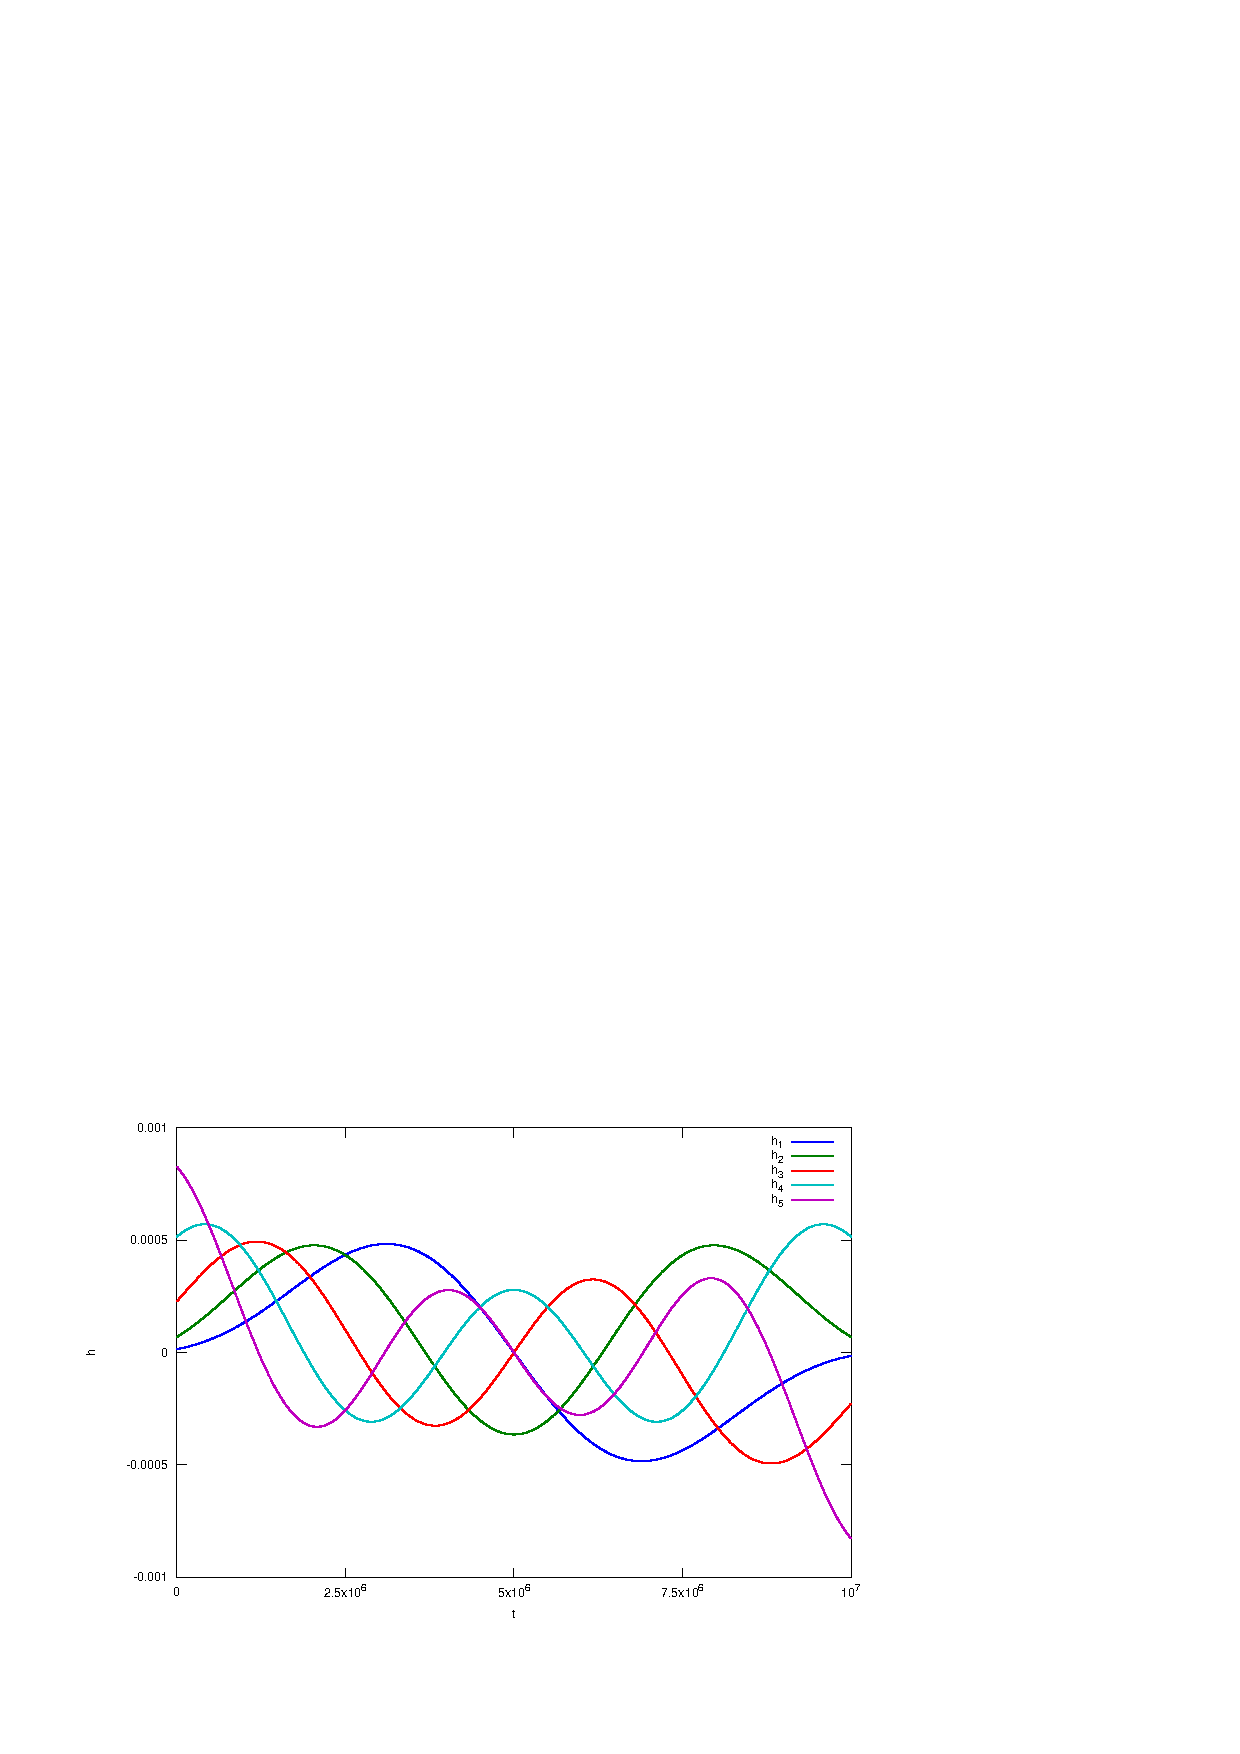
\includegraphics[width=0.9\textwidth]{pics/dpss1e+07.pdf}
    \vspace*{-0.5em}

    \caption[Advanced DPSS Example]{Discrete prolate spheroidal sequences computed in Listing \ref{lst:dpssadvanced}.\label{fig:dpssadvanced}}
    \vspace*{-0.5in}
\end{figure}

\index{dpss@\texttt{dpss}|)}
\clearpage

\newsection{Other Useful Routines \label{sec:otherroutines}}
There are several objects and routines that are used by one or both of \texttt{mtpsd} and \texttt{dpss}, but are not specific to either.  This includes applied statistics algorithms, basic error classes, and general mathematics operations that can be applied to many data types.  These are described in the section.

\subsection{ Applied Statistics: \texttt{applied\_stats.h}}

In order to find confidence intervals of a multitaper spectrum estimate, one must be able to compute percentage points (quantiles) of $\chi^2_\nu$ distributions.  Best and Roberts \cite{best:chisquared} have written a Fortran algorithm to accomplish this for arbitrary degrees of freedom $\nu$ and percentage point $p$.  The algorithm depends on a lower incomplete gamma function, and the percentage point of a Gaussian random variable.  A method to compute the incomplete gamma integral is given by Bhattacharjee \cite{bhatt:gamma}, and the quantiles of a Gaussian RV by Odeh and Evans \cite{odeh:normal}.  These three routines have been modified slightly and translated to C++.  They are defined in \code{applied_stats.h}, which is automatically included by \texttt{mtpsd.h}.
\medskip

\begin{lstshortblock}
double chisquared_inv( double p, double v )
void chisquared_inv( double p, double *v, unsigned int nv, double *x )
void chisquared_inv( double *p, double *v, unsigned int np, 
                     unsigned int nv, double *x )
\end{lstshortblock}
\begin{fdescription}
    Inputs: & \code{p, v}, (\code{np, nv})\\
    Outputs: & \code{x}\\
    & Computes the \code{p}$\times100\%$ percentage point of a $\chi^2_\nu$ distribution:
      \[P\left( \chi^2_\nu < x \right) = p.\]
      If \code{v} is an array of length \code{nv}, then the quantiles are stored in the array \code{x} (also of length \code{nv}).  If both \code{p} and \code{v} are arrays with respective lengths \code{np} and \code{nv}, then \code{x} is an \code{np}$\times$\code{nv} array in row-major format, where each row corresponds to the percentage points for a particular \code{p} and varying \code{v}.  The algorithm is based on Best and Roberts \cite{best:chisquared}.
\end{fdescription}\index{chisquared_inv@\texttt{chisquared\_inv()}}
\medskip

\begin{lstshortblock}
double gauss_inv(double p)
\end{lstshortblock}
\begin{fdescription}
    Inputs: & \code{p}\\
    & Computes the \code{p}$\times100\%$ percentage point of a standard Gaussian distribution with zero mean and unit variance: 
      \[P\left( \mathcal{N}(0,1) < x \right) = p.\]
      The algorithm is based on Odeh and Evans \cite{odeh:normal}.
\end{fdescription}\index{gauss_inv@\texttt{gauss\_inv()}}
\fdbottom
\newpage

\begin{lstshortblock}
double gamma_int(double x, double n)
double gamma_int_series(double x, double n)
double gamma_int_fraction(double x, double n)
\end{lstshortblock}
\begin{fdescription}
    Inputs: & \code{x, n}\\
    & Computes the incomplete gamma integral
    \[I(x,n)=\dfrac{1}{\Gamma(n)}\int_0^x e^{-t}t^{n-1}dt\]
    using either a polynomial series expansion (\code{_series}) or continued fractions (\code{_fraction}).  The unspecialized \code{gamma_int} automatically selects which version to use based on the inputs.  This algorithm is based on Bhattacharjee \cite{bhatt:gamma}.
\end{fdescription}\index{gamma_int@\texttt{gamma\_int()}}
\fdbottom
\vspace*{-0.5em}

\subsection{ The Simple Error Class: \texttt{simple\_error.h} \label{sec:simpleerr}}

Both the \texttt{dpss} and \texttt{mtpsd} libraries make use of the basic error class: \code{LAPACK_ERROR}, which is a child of \code{ERR}.  Specifically, the two eigenvalue routines \code{eig_rrr()}\index{eig\_rrr@\texttt{eig\_rrr()}} and \code{eig_iit()}\index{eig\_iit@\texttt{eig\_iit()}} throw an \code{LAPACK_ERROR} if the error status of the respective LAPACK routines is non-zero.  This error contains a brief message indicating the specific procedure that failed.  An error from one of these two routines will propagate down to the following:
\begin{verbatim}
    dpss_calc( ... )
    dpss::compute()
    mtpsd::compute()
\end{verbatim}
\index{dpss class@\texttt  {dpss} class!compute@\texttt{compute()}}\index{mtpsd class@\texttt  {mtpsd} class!compute@\texttt{compute()}}\index{dpss\_calc@\texttt{dpss\_calc()}}
Thus, if you wish to gracefully handle the error, these three routines should be contained within \code{try} blocks.  \code{LAPACK_ERROR} is derived from the \code{ERR} class, so both can be caught with \code{catch(ERR)}.  Listing \ref{lst:simpleerr} shows the definition of the two classes.
\smallskip

\begin{lstlisting}[label=lst:simpleerr,caption=The simple error classes ]
// Basic error class
class ERR{
    ERR();
    ERR(const char *msg);       //sets error message
    void getmsg(char *errmsg);  //copies error message to errmsg
    const char *getmsg();       //returns pointer to error message
};

// Inherits from ERR
class LAPACK_ERROR : public ERR{
    LAPACK_ERROR();
    LAPACK_ERROR(const char *errmsg);
};
\end{lstlisting} \index{ERR class@\texttt{ERR} class}\index{LAPACK_ERROR class@\texttt{LAPACK\_ERROR} class}
\medskip

\noindent One of these simple errors can be thrown with: \lstquick{throw ERR("My error message")}.


\subsection{General Mathematics Templates: \texttt{template\_math.h}}

Some general mathematics routines are needed by both the \texttt{mtpsd} and \texttt{dpss} libraries, and need to be able to handle a variety of input types.  These are written in the header \texttt{template\_math.h}, which is automatically included by both \texttt{mtpsd.h} and \texttt{dpss.h}.  Table \ref{tbl:templatemath} lists all the available functions, as well as a brief description of each.
\bigskip

\begin{table}[!hb]
    \centering
    \caption[Math template functions]{Description of the template functions in \texttt{template\_math.h}. \label{tbl:templatemath}}
    \vspace*{-0.5em}

    \noindent \begin{tabular}{@{}c@{}}
        \hline\hline\\
        \parbox{\textwidth}{
            \templatecode{template <class T>}{T}{abs( T a )}{Returns the maximum of +\code{a} and -\code{a}.  This does not compute a complex norm.}
            \templatecodecont{template <class T>}{T}{max( T a, T b )}{Returns the maximum of \code{a} and \code{b}.}
            \templatecodecont{template <class T>}{T}{min( T a, T b )}{Returns the minimum of \code{a} and \code{b}.}
            \templatecodecont{template <class T>}{T}{sum( const T *a, unsigned int n )}{ Returns the sum of the \code{n} elements in \code{a}.}
            \templatecodecont{template <class T>}{T}{mean( const T *a, unsigned int n )}{ Returns the mean of the \code{n} elements in \code{a}.  If \code{T} is an integer type, this mean will be truncated.}
            \templatecodecont{template <class T>}{double}{var( const T *a, unsigned int n )}{Returns the variance (second central moment) of the \code{n} elements in \code{a}.}\index{var@\texttt{var()}}
            \templatecodecont{template <class T>}{double}{mom2( const T *a, unsigned int n )}{Returns the second (non-central) moment of the \code{n} elements in \code{a}: $\sum\texttt{a[i]*}\overline{\texttt{a[i]}}/\texttt{n}$}\index{mom2@\texttt{mom2()}}
            \templatecodecont{template <class T>}{void}{scale( const T *a, double b, unsigned int n, T *ab)}{Scales the length-\code{n} array \code{a} by the constant \code{b}.  The result is stored in \code{ab}.}
            \templatecode{template <class A, class B>}{A}{wmean( const A *a, const B *wts, unsigned int n )}{ Returns the weighted mean: $\left(\sum\texttt{wts[i]}\right)^{-1}\sum\texttt{a[i]*wts[i]}.$\\  If \code{A} is an integer type, this mean will be truncated.}
            \templatecodecont{template <class A, class B>}{A}{dot\_mult( const A *a, const B *b, unsigned int n )}{ Returns the dot-product of the two length-\code{n} arrays \code{a} and \code{b}.}
            \templatecodecont{template <class A, class B>}{void}{pw\_mult( const A *a, const B *b, unsigned int n, A *ab )}{ Performs a point-wise multiplication of the two length-\code{n} arrays \code{a} and \code{b}.  The result is stored in \code{ab}.}
        }\\
        \hline
    \end{tabular}
\end{table}


\clearpage

\newsection{Octave Implementations \label{sec:octaveimp}}
\index{Octave dynamical extensions|(}

GNU \href{http://www.gnu.org/software/octave/}{Octave} is a very power computational tool for solving numerical problems.  It is most often compared to the widely used commercial product \textsc{Matlab}.  The two are mostly compatible when it comes to functions and scripts (m-files).  Octave has two major advantages:
\begin{itemize}
    \item Octave is free (as all academic tools should be).
    \item It is \emph{much} easier to program Octave dynamical extensions (oct-files) than \textsc{Matlab} executables (mex-files).
\end{itemize}
As with any open-source software, there are also disadvantages.  Not all the toolboxes available in \textsc{Matlab} have an equivalent in Octave.  Also, the support community is much smaller (although, for many problems, the \textsc{Matlab} solutions will work).

In order to use the multitaper libraries in Octave, two dynamical extensions are provided: \texttt{mtpsd.oct} and \texttt{dpss.oct}.  These are written to be replacements of the \code{pmtm.m} and \code{dpss.m} functions in \textsc{Matlab}'s Signal Processing Toolbox.  

\texttt{dpss.oct} is mostly compatible with \texttt{dpss.m}, with the exception of \textsc{Matlab}'s user-created database.  In \textsc{Matlab}, the interpolation routine selects a sequence from a user-created database as the base, whereas in this Octave version, the base sequence is always computed.  The syntax for both, however, is the same.  Both use the tridiagonal formulation, although \texttt{dpss.m} does not apply the even-odd splitting technique.  This Octave implementation has been found to be faster and more accurate (smaller $\|Ah_k-\lambda_kh_k\|$) than \textsc{Matlab}'s \texttt{dpss.m}, even at sizes as great as $2^{20}$, where it uses spline interpolation to generate the sequences.

\texttt{mtpsd.oct} is \emph{not} compatible with \texttt{pmtm.m}.  This was a design choice because the two methods have different features.  By default, \texttt{mtpsd} will remove weighted means to reduce bias, but \texttt{pmtm} will not.  \texttt{mtpsd} will \emph{always} return a two-side spectrum, whereas \texttt{pmtm} will return a one-side spectrum if the data is real.  The F-test can be performed by \texttt{mtpsd}, but not by \texttt{pmtm}.  Also, there are issues with \code{pmtm} when non-equal weights are used (see the Preface for details).  These are corrected in \code{mtpsd}.

The following two sections give the help files for \texttt{mtpsd.oct} and \texttt{dpss.oct}.  These can also be accessed using the \code{help} command in Octave.

\subsection{\texttt{mtpsd.oct}}

\index{mtpsd@\texttt{mtpsd}!Octave extension|(}
\deftypefn  {Loadable Function} {\var{S} =} {mtpsd (\var{x}, \var{nW}) }
\deftypefnx {Loadable Function} {\var{S} =} {mtpsd (\var{x}, \var{nW}, \var{nseq}) }
\deftypefnx {Loadable Function} {\var{S} =} {mtpsd (\var{x}, \var{nW}, \var{nseq}, \var{NFFT}) }
\deftypefnx {Loadable Function} {\var{S} =} {mtpsd (\var{x}, \var{nW}, \var{nseq}, \var{NFFT}, \var{Fs}) }
\deftypefnx {Loadable Function} {\var{S} =} {mtpsd (\var{x}, \var{nW}, \var{nseq}, \var{NFFT}, \var{Fs}, \var{pc}) }
\deftypefnx {Loadable Function} {\var{S} =} {mtpsd (\var{x}, \var{nW}, \var{nseq}, \var{NFFT}, \var{Fs}, \var{pc}, \var{pf}) }
\deftypefnx {Loadable Function} {\var{S} =} {mtpsd (\var{x}, \var{h}, \var{l}) }
\deftypefnx {Loadable Function} {\var{S} =} {mtpsd (\var{x}, \var{h}, \var{l}, \var{NFFT}) }
\deftypefnx {Loadable Function} {\var{S} =} {mtpsd (\var{x}, \var{h}, \var{l}, \var{NFFT}, \var{Fs}) }
\deftypefnx {Loadable Function} {\var{S} =} {mtpsd (\var{x}, \var{h}, \var{l}, \var{NFFT}, \var{Fs}, \var{pc}) }
\deftypefnx {Loadable Function} {\var{S} =} {mtpsd (\var{x}, \var{h}, \var{l}, \var{NFFT}, \var{Fs}, \var{pc}, \var{pf}) }
\deftypefnx {Loadable Function} {\var{S} =} {mtpsd (\dots{}, \var{'method'}) }
\deftypefnx {Loadable Function} {\var{S} =} {mtpsd (\dots{}, \var{'mean'}) }
\deftypefnx {Loadable Function} {[\var{S}, \var{f}, \var{Sc}, \var{FT}, \var{Jk}, \var{wk}, \var{h}, \var{l}] =} {mtpsd (\dots{}) }
\vspace{-0.5em}

\noindent Uses Thomson's Multitaper (MT) method to estimate the Power Spectral Density (PSD) of a one-dimensional time-series. The method uses orthogonal tapers to obtain a set of uncorrelated spectrum estimates, called eigenspectra.  These are then combined either linearly (equal or eigenvalue weighting), or non-linearly (adaptive weighting) to form a single spectrum. The resulting estimate has been shown to have lower variance and broad-band bias properties than the classical periodogram [1]. 

The data tapers are taken to be discrete prolate spheroidal sequences because of their desirable frequency characteristics. These sequences can be specified by their time-bandwidth product, \var{nW}, or can be supplied as column vectors of \var{h} with corresponding energy concentrations \var{l}.  The larger the value of \var{nW}, the larger the main lobe of the spectral windows.  See the \code{dpss} documentation for more details regarding their definition and calculation.

A particular weighting method for the multitaper estimate can be specified by the \var{'method'} string, which can take the following values:
\begin{texitable}
    \item[\var{'equal'}] Each eigenspectrum is weighted equally.
    \item[\var{'eigen'}] Each eigenspectrum is weighted by their energy concentration (eigenvalue).
    \item[\var{'adapt'}] Thomson's adaptive weighting is used, minimizing the broad-band bias.
\end{texitable}
By default, \code{mtpsd} will use adaptive weighting.

A confidence interval is computed if \var{Sc} is requested.  This interval is based on the assumption that the spectrum estimate follows a scaled chi-squared distribution, where the degrees of freedom is dependent on the eigenspectrum weights.  The width of the interval can be specified by the probability value \code{pc}.

An F-test for significant frequencies is computed if \var{FT} is requested.  The significance level can be set with the probability value \var{pf}.  Note: for non-equal weightings, the implemented F-test is a modified version of that described in [1].  It has been generalized to include the non-equal weights. See the \code{mtpsd} library documentation [2] for further details.

In order to reduce bias effects from constant terms, weighted means of the data are removed prior to computing each eigenspectrum.  These are never re-introduced, leaving estimation of the mean up to the user.  This behaviour can be overridden by including \var{'mean'} as the final input variable.
\bigskip

\noindent Input Variables:
\begin{texitable}
\item[\var{x}] One-dimensional time-series data (real or complex) of which to compute the power spectral density.
\item[\var{nW}] The time-bandwidth product for the DPSSs.  Typical values are 2, 2.5, 3, 3.5 and 4.
\item[\var{nseq}] The number of tapers to use.  The default value is $\lfloor 2nW \rfloor - 1$, since this is the number of DPSSs with energy concentrations close to one.
\item[\var{NFFT}] The length of the FFT used in spectrum calculations.  The returned spectrum will consist of \var{NFFT} values at equally spaced frequencies.  The default value is \code{length}(\var{x}).
\item[\var{Fs}] The sampling frequency.  The returned spectrum is evaluated in the Nyquist range [-Fs/2, Fs/2], beginning with the zero-frequency.  The default value is \var{Fs}=1.
\item[\var{pc}] The width of the confidence interval.  The output \var{Sc} corresponds to the lower and upper limits of the $pc\times100$\% confidence interval, assuming \var{S} follows a scaled chi-squared distribution.  The default value is \var{pc}=0.95.
\item[\var{pf}] The acceptance probability for the F-test.  If the F-statistic at a particular frequency exceeds the threshold, then the null-hypothesis (that the spectrum at f is caused by noise) is rejected at the $(1-pf)\times100$\% level. This indicates that the frequency is significant.  The default value is \var{pf}=0.95.
\item [\var{h}] User-supplied data tapers.  These are typically the first few discrete prolate spheroidal sequences, and can be computed using the \code{dpss} function.  They must have the same length as the time-series, \var{x}.  Tapers are taken to be the columns of \var{h}.
\item [\var{l}] Vector of energy concentrations for the user-supplied tapers.  This must have \var{nseq} entries, where \var{nseq} is the number of columns in \var{h}.  By definition, \var{l}(i) is the ratio of power in [-W, W] to total power for the i-th taper, where W is a normalized frequency defined by \var{nW}/\code{length}(\var{x}). 
\item [\var{'method'}] The weight method used to combine the individual eigenspectra into a single estimate.  Valid entries are: \var{'equal'}, \var{'eigen'}, and \var{'adapt'}.
\item [\var{'mean'}]  If specified, leaves the mean value in the data when computing the spectrum.  Otherwise, weighted means are removed (weighted by the tapers) prior to computing each eigenspectrum.  This is done to force the zero-frequency component to zero, eliminating any bias caused by constant terms.
\end{texitable}

\noindent If the empty vector, \code{[]}, is used for \var{nseq}, \var{NFFT}, \var{Fs}, \var{pc}, or \var{pf}, the default value is used.
\bigskip

\noindent Output Variables:

\begin{texitable}
    \item [\var{S}] The two-sided power spectral density estimate.  \var{S}(1) corresponds to the zero-frequency value.
    \item [\var{f}] Vector of frequencies.  \var{f} is in the range [0, \var{Fs}].
    \item [\var{Sc}] Confidence interval.  The first and second columns are the lower and upper bounds of the $pc\times100$\% confidence interval, respectively.  It is assumed that \var{S} follows a scaled chi-squared distribution.
    \item [\var{FT}] The F-test results.  The first column is the F-statistic assuming the spectrum at each frequency is composed of noise, and the second column is the $pf\times100$\% acceptance threshold.  If \var{FT}(i,1) $>$ \var{FT}(i,2), then the i-th frequency is significant.  If adaptive weighting is used, the threshold may return \code{Inf}.  This occurs when the spectrum estimate is deemed to be strongly biased, and is based almost entirely on a single eigenspectrum.  Since they are dominated by bias, these frequencies are not significant, so the F-test still functions as expected.
    \item [\var{Jk}]  The eigencoefficients.  These are formed by tapering the data and applying the FFT.  The eigenspectra are computed by squaring the complex norm: \var{Sk}=$\|$\var{Jk}$\|^2$.
    \item [\var{wk}] The weight vectors.  \var{wk} has dimensions \var{NFFT}$\times$\var{nseq}.  The i-th row is the set of weights used to calculate the i-th value of the spectrum: \var{S}$(i)=\sum_k$\var{wk}$(i)\|$\var{Jk}$(i)\|^2$. 
    \item [\var{h}] The data tapers, as columns.
    \item [\var{l}] Row vector containing the energy concentrations of the tapers.
\end{texitable}
\bigskip

\noindent Examples:
\medskip

\noindent Construct a periodic sequence with noise and plot its spectrum:
\begin{texiexample}
    Fs= 60;
    t = 0:1/Fs:5;
    x = cos(2*pi*20*t) + 0.2*randn(size(t));
    [S1,f,Sc1] = mtpsd( x,2.5,[],2*length(t),Fs);
    figure(1);
    plot( f, 10*log10([S1, Sc1]) );
\end{texiexample}
Here, adaptive weighting is used with the default \var{nseq} = 4 tapers.
\medskip

\noindent Perform an F-test for significant frequencies:
\begin{texiexample}
    [S2,f,Sc2,F] = mtpsd( x,2.5,[],2*length(t),Fs,[],1-1/length(x));
    fsig = f( F(:,1)>F(:,2) ); 
    printf('Significant frequencies:\t');
    disp(fsig');
\end{texiexample}
The frequencies in \code{fsig} surpass the the F-test threshold probability of 99.67\%.
\medskip

\noindent Spectrum of a complex series:
\begin{texiexample}
    z = exp(I*2*pi*20*t) + 1/sqrt(2)*(1+I);
    z = z+0.2*( randn(size(t)) + I*randn(size(t)) );
    S3a = mtpsd( z,2.5,[],2*length(t),Fs, 'eigen', 'mean');
    S3b = mtpsd( z,2.5,[],2*length(t),Fs, 'eigen');
    figure(2);
    plot( f, 10*log10([S3a S3b]) ); 
\end{texiexample}
In S3a, the mean is left in the data for spectrum calculations.  It is removed in the computation of S3b.
\bigskip

\noindent REFERENCES
\medskip

\noindent [1] Percival, D.B., and A.T. Walden, Spectral Analysis for Physical Applications: Multitaper and Conventional Univariate Techniques, Cambridge University Press, 1993.
\smallskip

\noindent [2] Sanchez, C.A., \code{mtpsd} Documentation, $<$http://sourceforge.net/projects/mtpsd$>$, 2010.
\index{mtpsd@\texttt{mtpsd}!Octave extension|)}

\subsection{\texttt{dpss.oct}}

\index{dpss@\texttt{dpss}!Octave extension|(}
\deftypefn  {Loadable Function} {\var{h} =}{dpss (\var{n},\var{nW})}
\deftypefnx {Loadable Function} {\var{h} =} {dpss (\var{n}, \var{nW}, \var{nseq})}
\deftypefnx {Loadable Function} {\var{h} =} {dpss (\var{n}, \var{nW}, \var{nseq}, \var{'interp'})}
\deftypefnx {Loadable Function} {\var{h} =} {dpss (\var{n}, \var{nW}, \var{nseq}, \var{'interp'}, \var{nb})}
\deftypefnx {Loadable Function} {\var{h} =} {dpss (\var{n}, \var{nW}, \var{'interp'})}
\deftypefnx {Loadable Function} {\var{h} =} {dpss (\var{n}, \var{nW}, \var{'interp'}, \var{nb})}
\deftypefnx {Loadable Function} {\var{h} =} {dpss (\dots{}, \var{'trace'})}
\deftypefnx {Loadable Function} {[ \var{h}, \var{l} ] =} {dpss (\dots{})}
\vspace*{-0.5em}

\noindent Computes a set of discrete prolate spheroidal sequences (aka Slepian sequences) using the symmetric tridiagonal matrix formulation, with even-odd splitting.  These sequences are typically used in multitaper spectral analysis.

The columns of \var{h} are the resulting sequences of length \var{n} and time-bandwidth product \var{nW}.  Typical values of \var{nW} are 2, 2.5, 3, 3.5 and 4.  The output \var{l} is a column vector containing the concentration of energy of each sequence in the normalized frequency range $f \in [-W,W]$.  By definition, the first discrete prolate spheroidal sequence maximizes this energy concentration.  The i-th sequence is the one that maximizes the concentration, subject to lying in the subspace perpendicular to that spanned by the previous i-1 sequences.  The initial $\lfloor 2nW \rfloor$ DPSSs have concentrations near one.  After this point, the concentrations rapidly drop to zero.

If \var{nseq} is not provided, then first $\lfloor 2nW \rfloor$ sequences are returned.  If \var{nseq} is an integer, $1\;\le$ \var{nseq} $ \le$ \var{n}, then the first \var{nseq} sequences are returned.  If \var{nseq} = [\var{seql}, \var{sequ}] is a range, then the \var{seql}-th through \var{sequ}-th sequences are returned.  Note: the first sequence has an index equal to one.

The maximum sequence length that can be calculated from the definition in this routine is \var{NMAX} = $2^{17}-1$.  For larger values of \var{n}, the DPSSs are approximated using interpolation.  Valid strings for \var{'interp'} are:
\begin{texitable}
    \item [\var{'spline'}] Interpolate using natural cubic splines (default).
    \item [\var{'linear'}] Interpolate linearly.
\end{texitable}
By default, sequences of length \var{n} $>$ \var{NMAX} are interpolated from the set of sequences generated by
\begin{texiexample}
    dpss ( NMAX, nW, ... ).
\end{texiexample}
\noindent If a base size, \var{nb}, is supplied, then the sequences are interpolated from
\begin{texiexample}
    dpss ( min (nb, NMAX), nW, ... ).
\end{texiexample}
\noindent The interpolation routine assumes that the sequences are evaluations of a function at the midpoints of an equally-spaced grid.  For the natural cubic splines, a zero-derivative boundary condition is assumed at the two end-points.

A final input string \var{'trace'} will print the interpolation method (if any) and the computation parameters to the command window.
\bigskip

\noindent Examples:
\medskip

\noindent Compute basic DPSSs:
\begin{texiexample}
    h = dpss(12, 3, 2); 
\end{texiexample}
The first two sequences with length 12 and time-bandwidth product \var{nW}=3 are returned.
\medskip

\noindent Compute a range of DPSSs:
\begin{texiexample}
    h = dpss(12, 3, [3 5]); 
\end{texiexample}
The third through fifth DPSSs of length 12 and \var{nW}=3 are returned.
\medskip

\noindent Use interpolation to compute long sequences:
\begin{texiexample}
    [h, l] = dpss(8388608, 2.5, 'spline', 32768); 
\end{texiexample}
\noindent The first 2\var{nW}=5 sequences of length $2^{23}$ and time-bandwidth product \var{nW}=2.5 are returned, along with their energy concentrations.  Note that these were obtained by first computing sequences of length $2^{15}$, then interpolating using natural cubic splines and re-normalizing to have unit energy.  The interpolated sequences are used to estimate the energy concentrations.

\index{dpss@\texttt{dpss}!Octave extension|)}

\index{Octave dynamical extensions|)}

\newpage

\newsection{Command-Line Implementation \label{sec:cmdimp}}
\index{dpss@\texttt{dpss}!executable}
Currently, only the \texttt{dpss} module has been implemented as a command-line executable.  The binary prints the sequences and eigenvalues directly to the terminal.  On Unix-based systems, this output can be re-directed to a file in the standard way.  The format of the output is compatible with a \textsc{Matlab}/Octave script file, producing the two arrays: \code{dps_seq} for the sequences, and \code{lambda} for the eigenvalues.  The following is the help file, which can be accessed with \texttt{dpss --help}:
{\small
\begin{verbatim}
  Usage: dpss n nW [[seql] sequ] [interp_method [interp_base]] [trace]

  `dpss' calculates and prints a set of "discrete prolate spheroidal sequences"
  (aka Slepian Sequences) and their corresponding concentrations of energy in
  the normalized bandwidth [-W, W].  These sequences are typically used in 
  multitaper spectral analysis.

  Examples:
  dpss 12 3 2        returns the first two DPSSs of length 12 and time-bandwidth
                     product nW=3, along with their concentrations.
  dpss 12 3 3 5      returns the third through fifth DPSSs and concentrations.
  dpss 8388608 2.5 spline 32768   calculates the first five DPSSs of length 2^15,
                                  nW=2.5, then interpolates to length 2^23 using 
                                  natural cubic splines, re-normalizes and
                                  estimates the new energy concentrations.

  Required Parameters:
    n     Length of the dpss sequences to be computed
    nW    Time-bandwidth product for the sequences.  By definition, the first
          dpss maximizes the concentration of energy in the normalized frequency 
          range f in [-W,W]. Typical values are nW = 2, 2.5, 3, 3.5 and 4.

  Optional Parameters:
    sequ             The index of the upper dpss to be calculated.  Indices must
                     fall in the range [1, N].  If `seql' is not defined, then
                     this is the total number of sequences.  By default,
                     sequ = floor(2nW). 
    seql             The index of the lower dpss to be calculated.  This must
                     fall in the range [1, sequ].
    interp_method    Interpolation method to employ when creating the sequences.
                     By default, dpss will calculate sequences up to length
                     n = 2^17-1 without interpolation.  For larger sequences, 
                     intermediate values must be interpolated.  Accepted methods
                     are `linear' and `spline' (without quotes).  By default,
                     interp_method=spline, which uses natural cubic splines.
    interp_base      Length of the sequences from which to interpolate.  An 
                     interpolation method must be supplied to use this option.
                     By default, interp_base = min( n, 2^17-1 ).
    trace            trace = `trace' (without quotes) prints the method and 
                     computation parameters to the command window.

  See the `mtpsd' Documentation for further details.
\end{verbatim}
}

\newpage

\newsection{Contact}

Found a bug?  Something not working as expected?  As it should?  Questions?  Comments?  Feel free to contact the author:
\medskip

\indent Antonio S\'anchez\\
\indent \href{mailto:antonio@eigenspectrum.com}{antonio@eigenspectrum.com}

\newpage

\renewcommand{\sectiontitle}{References}
\markboth{\scshape \sectiontitle}{}
\pagestyle{contents}
\nocite{*}  %adds all titles in bib files to bibliography
%\bibliographystyle{plain}
\bibliographystyle{abbrvnat}
\bibliography{mtpsd}
\addcontentsline{toc}{section}{References}

{\small
\renewcommand{\sectiontitle}{Index}
\markboth{\scshape \sectiontitle}{}
\printindex
}

\end{document}
